% kate: word-wrap true;

% IMPORTANT NOTE: I've never dealt much with syntax before, at least not in a
% way as formal as I'm trying to come to terms with it here. If there's
% anything wrong with my analyses, it's because I don't know enough yet. Things
% may be subject to change *especially* in this chapter.

\chapter{Phrase structures}
\label{ch:phrasestruct}

While the previous chapter dealt largely with the various parts of speech and
their various distributive and inflectional properties, the present chapter
will elaborate on how these words combine into syntactic phrases. Since Ayeri
is a verb-initial language, it is probably most comfortably analyzed in terms
of Lexical-Functional Grammar (\cite{bresnan1982}~ff.; more recently
\cite{bresnan2016}; \cite{dalrymple2001}), since \Lfg{} does not require
complicated derivations behind the surface structure of
sentences.\footnote{Passivization, for instance, is assumed to be a lexically
motivated alternation in predicate structure (\Sbj{} is blocked, so the
nominative is assigned to \Obj{}, and the original \Sbj{} is expressed  by an
\Adjc{}), rather than an internal derivational process
\citep[23\psqq]{bresnan2016}.} It will be assumed here that, even though Ayeri
is basically VSO with predicate and predication not adjacent to each other, it
is configurational in that there is a VP which c-commands a number of other
constituents as complements in transitive sentences.

In principle, \Lfg{} assumes that grammar operates on different structural 
levels: mainly, these are a(rgument) structure, c(onstituent) structure, and 
f(unctional) structure; other layers have been proposed by different 
researchers for different purposes \citep[862--865]{buttking2015}. 
\citet{bresnan2016} define three core design principles for \Lfg{}:

\begin{description}
\item[Variability:] \textcquote[41]{bresnan2016}{The principle of variability
states that \emph{external structures vary across languages}. The formal model
of external structure in \Lfg{} is the \emph{c-structure}, which stands for
\enquote{constituent structure} or \enquote{categorial structure}}. 
C-structures are commonly represented by context-free phrase-structure rules; 
constituency trees are based on an extended version of X-bar theory 
\citep[42]{bresnan2016}.\footnote{The basic recursive rules of X-bar theory 
are observed:
\begin{enumerate}[nosep, leftmargin={2\footnotemargin}]
\item XP → YP, \xbar{X} (specifier rule)
\item \xbar{X} → \xbar{X}, YP (adjunct rule)
\item \xbar{X} → \xhead{X}, YP (complement rule)
\end{enumerate}

The principle of economy of expression furthermore dictates that essentially, 
trees be pruned of empty terminal nodes and non-branching preterminal nodes, 
since these do not provide structurally or semantically relevant information 
\citep[119--128]{bresnan2016}.}

\item[Universality:] \textcquote[42]{bresnan2016}{The principle of universality
states that \emph{internal structures are largely invariant across languages}.
The formal model of internal structure in \Lfg{} is the \emph{f-structure},
which stands for \enquote{functional structure}}. The f-structure is depicted
as an argument-value matrix (\Avm{}) which maps the relations between `subject'
(\Sbj{}), `object' (\Obj{}), `predicator' (\Pred{}), etc.\ as functional
abstractions of NP, VP, V, etc.\ \citep[42]{bresnan2016}. Verbs are also
presented with their \fw{a-structure} spelled out. That is, which arguments a
verb has relations to is formally stated \citep[15]{bresnan2016}. The
f-structure collates semantic features associated with heads of grammatical
functions (GFs), such as case (\Case{}), person (\Pers{}), number (\Num{}),
which are abstract features and as such need not have morphological realization
\citep[43]{bresnan2016}.

\item[Monotonicity:] \textcquote[43]{bresnan2016}{Constituent structure form is
simply not the same in all languages [...] In \Lfg{} the correspondence mapping
between internal and external structures does not preserve sameness of form.
Instead, \emph{it is designed to preserve inclusion relations between the
information expressed by the external structure and the content of the internal
structure}}. Due to the principle of monorepresentation, information
distributed over different morphemes which logically belongs to a single
grammatical function is presented in the f-structure as unified.

\end{description}

\begin{figure}[t]\centering
\begin{tabular}[t]{l @{\quad\quad} c}
argument (a-)structure:
& \astruct{\tikzmark{verb}verb}{\tikzmark{x}x, \tikzmark{y}y}\bigskip \\

functional (f-)strucutre:
& \tikzmark{fstruct}{\smaller\begin{avm}
\[
	\quad sbj \tikzmark{subj} & \[
		{\enspace}\vdots{\enspace} \\
	\]{\quad} \\
	
	\quad obj \tikzmark{obj} & \[
		{\enspace}\vdots{\enspace} \\
	\] \tikzmark{objval}{\quad} \\
	\quad \tikzmark{pred} pred & \dots \tikzmark{predval} \\
\]
\end{avm}}\bigskip\\

constituent (c-)structure:
& \begin{forest} baseline
[\xbar{V}
	[\subnode{V}{V}]
	[NP \tikzmark{NP}
		[\xbar{N} \tikzmark{Nbar}]
	]
]
\end{forest}
%
\end{tabular}
\begin{tikzpicture}[remember picture, overlay]
\draw [-latex]
	([xshift=1.5ex, yshift=-0.5ex]{pic cs:verb})
	to [out=south, in=north west]
	([yshift=1ex]{pic cs:pred});
	
\draw [-latex]
	([xshift=0.5ex, yshift=-0.5ex]{pic cs:x})
	to [out=south, in=north east]
	([yshift=1ex]{pic cs:subj});
	
\draw [-latex]
	([xshift=0.5ex, yshift=-0.75ex]{pic cs:y})
	to [out=south, in=north east]
	([yshift=1ex]{pic cs:obj});
	
\draw [-latex]
	([yshift=1ex]{pic cs:V})
	to [out=west, in=south west]
	([yshift=-10ex]{pic cs:fstruct});
	
\draw [-latex]
	([yshift=1ex]{pic cs:NP})
	to [out=east, in=east]
	([yshift=1ex]{pic cs:objval});
	
\draw [-latex]
	([yshift=1ex]{pic cs:Nbar})
	to [out=east, in=east]
	([yshift=1ex]{pic cs:objval});
\end{tikzpicture}
\caption[F-structure mappings]{F-structure mappings \citep[15]{bresnan2016}}
\label{fig:phimap}
\end{figure}

To illustrate the different parallel structures in operation,
\citet[15]{bresnan2016} give the schema in \autoref{fig:phimap} to demonstrate
which part of the a- and c-structure respectively corresponds (`links', `maps')
to which part of the f-structure.
% \footnote{\citet{bresnan2016} use \textsc{`subj'} for `subject'. ; for
% consistency with the above I will use `\Sbj{}' in the following. I will also
% divergently use \Compl{} and \XCompl{} for \textsc{(x)comp}, since
% \textsc{comp} has already been used for `comparative' above.}
Regarding the different functions distinguished, \Lfg{} 
assumes the following hierarchies \citep[97, 100]{bresnan2016}:

\pex\label{ex:functions}
\a\label{ex:gfs} Grammatical functions (\GF{}s):\\
	$\overbrace{\Sbj{} > \Obj{} > \SObj{}}^{\text{core}} > 
	\overbrace{\Oblique{} > \XCompl{}, \Compl{} > \Adjc{}}^{\text{noncore}}$
\a\label{ex:nonafs} (Non)argument functions (\AF{}s/$\overline{\mbox{\AF{}}%
}$s):\\
	$\underbrace{\Top{}\: \Foc{}}_{\text{non-a-fns}}\; 
	\overbrace{\Sbj{}\: \Obj{}\: \SObj{}\: \Oblique{}\: \XCompl{}\: 
		\Compl{}}^{\text{a-fns}}\; 
	\underbrace{\Adjc{}}_{\text{non-a-fns}}$
\a\label{ex:dfs} Discourse functions (\DF{}s):\\
	$\overbrace{\Top{}\: \Foc{}\: \Sbj{}}^{\text{d-fns}}\;  
	\underbrace{\Obj{}\: \SObj{}\: \Oblique{}\: \XCompl{}\: \Compl{}\: 
		\Adjc{}}_{\text{non-d-fns}}$
\xe

The elements listed in (\ref{ex:functions}) will also appear in
phrase-structure rules and c-structure trees together with arrows. These arrows
symbolize inheritance of feature information from the current level (↓) of the
tree to the next (↑), so for instance, `\pass{\Sbj}' means that the information
subsumed by the current node (`down') is passed on as the subject function of
the next higher node (`up') in the tree. Concise information on notational
formalisms of \Lfg{} can be found, for instance, in \citet{buttking2015}.

\section{Noun phrases and determiner phrases}
\label{sec:nps-dps}

Noun phrases (NPs), and determiner phrases (DPs) as their functional 
counterpart, fulfill the functions of subject (\Sbj{}), object (\Obj{}), 
secondary object (\SObj{}), as well as various oblique constituents (\Oblique;
see (\ref{ex:dpnpcasemap}) below), and they can also form adjuncts (\Adjc{}).
DPs and NPs can also constitute topics (\Top{}). Which DP or NP receives which 
function is selected by the a-structure of the verb---this also has 
repercussions on case- and topic marking.

Since the constituent containing the various non-verbal elements in Ayeri is 
likely exocentric and constituents may move around within it in a restricted 
way, we have to assume that not constituent structure, but case marking 
identifies the grammatical functions of the various arguments of verbs. Thus, 
the following lexicocentric conditions operate on both DP and NP as exponents 
of case:

\ex\label{ex:dpnpcasemap}\labels
\begin{tabular}[t]{@{} l @{\quad} l @{$\implies$} l}
\tl\quad & \downs{\Case} = \Aarg	& \pass{\Sbj} \\
\tl\quad & \downs{\Case} = \Parg	& \pass{\Obj} \\
\tl\quad & \downs{\Case} = \Dat		& \pass{\SObj} \logor{}
	\pass{\Oblq{to}} \\
\tl\quad & \downs{\Case} = \Gen		& \pass{\Possr} \logor{} 
	\pass{\Oblq{src}} \logor{} \pass{\Oblq{from}} \\
\tl\quad & \downs{\Case} = \Loc		& \pass{\Oblq{loc}} \\
\tl\quad & \downs{\Case} = \Caus	& \pass{\Oblq{caus}} \\
\tl\quad & \downs{\Case} = \Ins		& \pass{\Oblq{ins}} \\
\end{tabular}
\xe

The rules in (\ref{ex:dpnpcasemap}) determine the typical mappings between case
marking and grammatical functions, which are not always unambiguous. As
explained above (compare \autoref{subsec:case}), the dative case does not only
indicate that something is done to this referent or to their benefit, but it
may also indicate motion towards this referent. Likewise, the genitive case
does not only indicate possession, but also origin, and motion from this
referent. Nominal adjuncts to nouns which specify what the noun consists also
appear in the instrumental case, besides the instrumental being used to
indicate the means or the circumstance by which an action comes about.
Moreover, DPs or NPs may also lack case marking, which indicates that the
respective phrase is a part of the topic of the verb, which is what
(\ref{ex:topicrule}) describes:

\ex\label{ex:topicrule}
¬\,\downs{\Case} $\implies$ \elem{\Top}
\xe

Instead of case marking on the DP or NP, there is a marker in front of the verb
which provides information on the case and, if \AgtT{} or \PatT{}, also about
the animacy of the topicalized phrase. This means that grammatical information
about the topic of a phrase is spread over two discontinuous locations. This
issue does not pose a problem to an \Lfg{}-based analysis, however, since both
locations unify their information content in the f-structure feature \Top{}.
Since information located in multiple places is jointly feeding this feature, I
am using the annotation `\elem{\Top}' for each location rather than simple
`\pass{\Top}'. Note that only one NP among the arguments of a verb may be the
topic of the phrase, and a topic can only be marked if the verb is finite and
the number of arguments to the verb is greater than one.

\subsection{Noun phrases}
\label{subsec:nps}

\subsubsection{Constituent order within noun phrases}

Nouns are one of the main parts of speech of Ayeri, and nouns can be modified
by a number of other free elements, as we have seen previously---adjectives,
possessive adjectives, as well as relative clauses and nominal adjuncts. These
typically follow nouns. It was also described before that Ayeri's nouns may
host a number of clitics, among which are deictic prefixes and quantifiers, as
well as enclitic case markers in the case of proper nouns. These clitics,
however, will not be treated as targets of syntactic operations, since \Lfg{}
follows the approach of lexical integrity. Thus, bound elements like affixes
and clitics are assumed not to be reflected or affected by syntax itself. The
phrase structure of NPs should thus look like depicted in (\ref{ex:npstruct}).

\pex\label{ex:npstruct}
\a NP → \anno*{\xbar{N}}
\a \xbar{N} → \anno*{\xhead{N}} $\left(\anno*[{\pass{\Adjc}}]{XP}\right)$
\xe

This rule defines that NPs have a lexical head which is on the left side,
followed optionally by modifiers which act as adjuncts to the noun. The
description leaves open which kind of phrases the adjuncts can consist of, but
as mentioned above, these are commonly adjectives (forming adjective phrases,
APs), nominal adjuncts (NPs), as well as relative clauses (forming
complementizer phrases, CPs). This can be represented as a
constituent-structure tree in the way described in (\ref{ex:npcstruct}).

\ex\label{ex:npcstruct}\labels
\begin{forest}
[{\anno[\{\pass{df} | \pass{gf}\}]{NP}}
	[\anno{\xbar{N}}
		[\anno{\xhead{N}}]
		[{$\left(\anno[{%
				\pass{\Adjc}%
			}]{XP}\right)$
		}]
	]
]
\end{forest}
\xe

Here as well, we can see a nominal head on the left which may be modified by
adjuncts of various types. The maximal projection of \xhead{N} (that is, NP) is
annotated very generally for the function of the NP---basically, an NP can act
as either a discourse function (DF) or a grammatical function (\GF{}). 
(\ref{ex:nounmods}) gives an example of each kind of modifier. Since there is 
no grammatical context given, NP is unmarked for function in these examples.

\pex\label{ex:nounmods}
\a %
	\begin{minipage}[t]{.5\remaining}
	\begingl
		\glpreamble noun + adjective: //
		\gla ningan hiro //
		\glb ningan hiro //
		\glc story new //
		\glft `new story' //
	\endgl
	\end{minipage}
	~
	\begin{forest} shorter edges, italic leaves,
	[NP
		[\anno{\xbar{N}}
			[\anno{\xhead{N}}
				[{ningan}]
			]
			[{\anno[\pass{\Adjc}]{AP}}
				[{hiro}, roof]
			]
		]
	]
	\end{forest}

\a %
	\begin{minipage}[t]{.5\remaining}
	\begingl
		\glpreamble noun + possessor: //
		\gla kegan ayonena //
		\glb kegan ayon-ena //
		\glc hat man-\Gen{} //
		\glft `the man's hat' //
	\endgl
	\end{minipage}
	~
	\begin{forest} shorter edges, italic leaves,
	[NP
		[\anno{\xbar{N}}
			[\anno{\xhead{N}}
				[{kegan}]
			]
			[{\anno[\pass{\Possr}]{NP}}
				[{ayonena}, roof]
			]
		]
	]
	\end{forest}

\a %
	\begin{minipage}[t]{.5\remaining}
	\begingl
		\glpreamble noun + instrumental complement: //
		\gla kasu bariri //
		\glb kasu bari-ri //
		\glc basket meat-\Ins{} //
		\glft `basket of meat' //
	\endgl
	\end{minipage}
	~
	\begin{forest} shorter edges, italic leaves,
	[NP
		[\anno{\xbar{N}}
			[\anno{\xhead{N}}
				[{kasu}]
			]
			[{\anno[\pass{\Oblq{ins}}]{NP}}
				[{bariri}, roof]
			]
		]
	]
	\end{forest}

\a %
	\begin{minipage}[t]{.5\remaining}
	\begingl
		\glpreamble noun + relative clause: //
		\gla nanga si incāng //
		\glb nanga si int=yāng //
		\glc house \Rel{} buy=\TsgM{}.\Aarg{} //
		\glft `the house he bought' //
	\endgl
	\end{minipage}
	~
	\begin{forest} shorter edges, italic leaves,
	[NP
		[\anno{\xbar{N}}
			[\anno{\xhead{N}}
				[{nanga}]
			]
			[{\anno[\pass{\Compl}]{CP}}
				[{si incāng}, roof]
			]
		]
	]
	\end{forest}

\xe

As described before (compare \autoref{subsec:clitics}), nouns can be modified
by a number of clitics which are not represented through syntax. Since it is
not possible for these clitic elements to be divided from their phonological
hosts, they should be treated as being an integral part of the word they attach
to. Hence, \xhead{N} is given in (\ref{ex:nouncltree}) as split into `Cl' and
\xhead{N}.

\pex\label{ex:nouncltree}
\a %
	\begin{minipage}[t]{.5\remaining}
	\begingl
		\glpreamble noun + deictic prefix: //
		\gla eda- @ nanga //
		\glb eda= nanga //
		\glc this= house //
		\glft `this house' //
	\endgl
	\end{minipage}
	~
	\begin{forest} shorter edges, italic leaves,
	[\anno{\xhead{N}}
		[\anno{Cl}
			[eda-]
		]
		[\anno{\xhead{N}}
			[nanga]
		]
	]
	\end{forest}

\a %
	\begin{minipage}[t]{.5\remaining}
	\begingl
		\glpreamble noun + quantifier: //
		\gla nangās @ -ikan //
		\glb nanga-as =ikan //
		\glc house-\Parg{} =many //
		\glft `many houses' //
	\endgl
	\end{minipage}
	~
	\begin{forest} shorter edges, italic leaves,
	[\anno{\xhead{N}}
		[\anno{\xhead{N}}
			[nangās]
		]
		[\anno{Cl}
			[-ikan]
		]
	]
	\end{forest}

\a %
	\begin{minipage}[t]{.5\remaining}
	\begingl
		\glpreamble proper noun + case: //
		\gla ang @ Diyan //
		\glb ang= Diyan //
		\glc \Aarg{}= Diyan //
		\glft `Diyan' //
	\endgl
	\end{minipage}
	~
	\begin{forest} shorter edges, italic leaves,
	[\anno{\xhead{N}}
		[\anno{Cl}
			[ang]
		]
		[\anno{\xhead{N}}
			[Diyan]
		]
	]
	\end{forest}

\xe

Of course, it is also possible to combine these nominal modifiers. In this
case, there is a certain hierarchy, presumably based on Behaghel's first law,
\textquote{Das oberste Gesetz ist dieses, daß das geistig eng Zusammengehörige 
auch eng zusammengestellt wird} (\cite[4]{behaghel1932}; `The supreme law is
such that the mentally closely related is also arranged in close proximity.'), 
and also grammatical weight \citep{wasow1997}:

\begin{enumerate}[noitemsep]
	\item instrumental NP indicating what the head consists of,
	\item APs (also cardinals) and other NPs describing attributes,
	\item possessive genitive NPs,
	\item relative clauses.
\end{enumerate}

\citet{wasow1997} writes that \textcquote[102]{wasow1997}{[i]t is very hard to
distinguish among various structural weight measures as predictors of weight
effects. Counting words, nodes, or phrasal nodes all work well}, which means
that no single metric can be used to describe the order of constituents in a
phrase. However, for instance, relative clauses trail whenever possible
presumably since they tend to contain whole subclauses and thus a lot of
information. It seems advisable not to put an element with much less 
information content after them, especially when it refers to a different head
than all the things inside the relative clause. The following example 
(\ref{ex:nounmodord}) illustrates the unmarked order of modifiers.

\pex\label{ex:nounmodord}
\a\begingl
	\gla diranang caban nā si ang mica ya @ Kārvisam //
	\glb diran-ang caban nā si ang mit=ya.Ø ya= Kārvisam //
	\glc uncle-\Aarg{} favorite \Fsg{}.\Gen{} \Rel{} \AgtT{} 
		live=\TsgM{}.\Top{} \Loc{}= Kārvisam //
	\glft `my favorite uncle who lives in Kārvisam' //
\endgl
\medskip

\a\begin{forest} shorter edges, narrower nodes, italic leaves,
[{\anno[\pass{\Sbj}]{NP}}
	[\anno{\xbar{N}}
		[\anno{\xbar{N}}
			[\anno{\xbar{N}}
				[\anno{\xhead{N}}
					[{diranang}]
				]
				[{\anno[\pass{\Adj}]{AP}}
					[{caban}, roof]
				]
			]
			[{\anno[\pass{\Possr}]{DP}}
				[{nā}, roof]
			]
		]
		[{\anno[\pass{\Comp}]{CP}}
			[{si ang mica ...}, roof]
		]
	]
]
\end{forest}

\xe

As the c-structure tree in (\ref{ex:nounmodord}) shows, Ayeri prefers
head--dependent word order with exceeding consistency. As illustrated by
previous examples, both adjuncts and complements are, for the most part,
consistently appended to the right of their heads, which means that Ayeri may
be classified as a rather consistently right-branching language. However, a
certain number of postpositions form an exception to this classification
(\autoref{subsec:postpos}). In the light of word order typology, we can
formulate the following generalizations:

\pex
\a Order of noun and adjective: N Adj
\a Order of noun and genitive: N Gen
\a Order of noun and relative clause: N Rel
\xe

More important to \Lfg{} than c-structure trees, however, are
function-structure matrices which gather all information in a given utterance
and gather potentially disparate information into semantically coherent units
within the matrix.\footnote{Essentially, c-structure is similar to the tree
hierarchy of paragraphs, images, tables etc.\ in an \textsc{html} file, while
f-structure describes semantic properties of elements in the tree similar to
how \textsc{css} defines the layout properties of these elements.} In the
following, I will thus give a list of morpholexic specifications which give an
overview of the different semantic and morphological features nouns basically
provide (also compare \autoref{sec:nouns}). These also form the basis for
f-structure matrices of the kind already shown in (\ref{ex:clitics_43}),
\autoref{clitics_postverb_person}, p.~\pageref{ex:clitics_43}.

\begin{morphlex}
\ex\label{ex:nounmorphlex}%
\adjustbox{valign=t}{%
	\begin{tabu} {\usetabu{morphlexnarrow}}
	...
		& N
		& \begin{tabular}[t]{l l l}
			\ups{\Pred} & = & `...' \\
			\ups{\Anim} & = & $\pm$ \\
			\ups{\Case} & = & \{\Aarg{}, \Parg{}, \Dat{}, \Gen{}, 
				\Loc{}, \Ins{}, \Caus{}\} \\
			\ups{\Gend} & = & \{\M{}, \F{}, \N{}, \Inan{}\} \\
			\ups{\Num} & = & \{\Sg{}, \Pl{}\} \\
			\ups{\Pers} & = & 3 \\
		\end{tabular}
	\end{tabu}%
}
\xe
\end{morphlex}

Nouns generally imply a third-person reference; they distinguish number, gender
and animacy, as well as case. Clitics, however, may also add information about
deixis (\ref{ex:deixisfeat}); likeness and quantity might be interpreted
conveniently as adding to the list of a noun's \Adjc{} feature 
(\ref{ex:nounqadj}).

\begin{morphlex}
\ex\label{ex:deixisfeat}
\adjustbox{valign=t}{%
	\begin{tabu} {\usetabu{morphlexnarrow}}
	\hphantom{...}
		& \hphantom{N}
		& \begin{tabular}[t]{l l l}
			\ups{\Deix} & = & \{$this$, $that$, $such$\} \\
		\end{tabular}
	\end{tabu}%
}
\xe
\end{morphlex}

\pex~\label{ex:nounqadj}
\a\begingl
	\gla ganang-hen mino //
	\glb gan-ang=hen mino //
	\glc child-\Aarg{}=all happy //
	\glft `all happy children' //
\endgl

\a\begin{avm}
\[
	\Subj{}	&	\[
					\Pred	&	`child' \\
					\Anim	&	$+$ \\
					\Case	&	\Aarg \\
					\Adjc	&	\{
									\[
										\Pred	&	`all' \\
									\], \\
									\[
										\Pred	&	`happy' \\
									\] \\
								\} \\
				\] \\
\]
\end{avm}
\xe

\subsubsection{Morphosyntactic operations within the noun phrase}

It has been pointed out above that nouns encode animacy. This has repercussions
in the choice of case markers of the agent and patient cases, which need to
agree with the lexical head they attach to. An example of this is given in 
(\ref{ex:animcaseagr}).

\pex\label{ex:animcaseagr}
\a\label{ex:animok} %
\begin{forest}
[\anno{\xhead{N}}
	[\anno{N\tsub{stem}}
		[{%
			\textit{gan} \\
			\ups{\Anim} = $+$ \\
		}]
	]
	[\anno{-N\tsub{infl}}
		[{%
			\textit{-ang} \\
			\ups{\Anim} = $+$ \\
			\ups{\Case} = \Aarg{} \\
		}]
	]
]
\end{forest}

\a\label{ex:animclash} %
\ljudge*\begin{forest}
[\anno{\xhead{N}}
	[\anno{N\tsub{stem}}
		[{%
			\textit{gan} \\
			\ups{\Anim} = $+$ \\
		}]
	]
	[\anno{N\tsub{infl}}
		[{%
			\textit{-reng} \\
			\ups{\Anim} = $-$ \\
			\ups{\Case} = \Aarg{} \\
		}]
	]
]
\end{forest}
\xe

Example (\ref{ex:animok}) shows a well-formed construction: the noun,
\xayr{gnF}{gan}{child}, is animate, hence the case particle also needs to be 
animate---the case particle must thus be \rayr{/As}{-ang} to be coherent. In
contrast to this, example (\ref{ex:animclash}) is not well-formed in that the
noun is animate but the case particle, \rayr{/reNF}{-reng}, signals that it is
inanimate: the \Anim{} values of the noun stem and its suffix clash and cannot
be conclusively unified for \xhead{N} itself. The same principle of coherence
is, of course, also true for proper nouns, which receive a case-marking
particle:

\pex\label{ex:animcaseagrname}
\a\label{ex:animokname} %
\begin{forest}
[\anno{\xhead{N}}
	[\anno{Cl}
		[{%
			\textit{ang} \\
			\ups{\Anim} = $+$ \\
			\ups{\Case} = \Aarg{} \\
		}]
	]
	[\anno{\xhead{N}}
		[{%
			\textit{Dita} \\
			\ups{\Anim} = $+$ \\
		}]
	]
]
\end{forest}

\a\label{ex:animclashname} %
\ljudge*\begin{forest}
[\anno{\xhead{N}}
	[\anno{Cl}
		[{%
			\textit{eng} \\
			\ups{\Anim} = $-$ \\
			\ups{\Case} = \Aarg{} \\
		}]
	]
	[\anno{\xhead{N}}
		[{%
			\textit{Dita} \\
			\ups{\Anim} = $+$ \\
		}]
	]
]
\end{forest}
\xe

Furthermore, example (\ref{ex:nounqadj}) already showed that nouns may be
modified by quantifiers, whether these are clitic suffixes
(\autoref{subsec:quantifiers}) or numerals (\autoref{sec:numerals}). In these
cases, plural marking on the noun is suppressed by the presence of the modifier
which supplies the information by itself so that further morphological plural
marking by the suffix \rayr{/ye}{-ye} on the noun stem itself would be
redundant. As shown in \autoref{sec:numerals} (p.~\pageref{hundreds}), however,
there are very limited occasions where a noun may be marked for plural in spite
of the presence of a numeral, for instance:

\ex\begingl
	\gla Ang bengyon keynamye menang kanānya {desay iray}. //
	\glb ang beng-yon keynam-ye-Ø menang kanān-ya {desay iray} //
	\glc \AgtT{} attend-\TplN{} people-\Pl{}-\Top{} hundred wedding-\Loc{} 
		royal //
	\glft `Hundreds of people attended the royal wedding.' //
\endgl\xe

Here, the noun \xayr{kejnmF}{keynam}{people} is marked additionally for plural
by the nominal plural suffix \rayr{/ye}{-ye} in spite of being a \fw{plurale
tantum} and in spite of the presence of the numeral \rayr{menNF}{menang}
{hundred}. Without plural morphology, the meaning of \rayr{kejnmF menNF}{keynam
menang} would be `a hundred people', not generic `hundreds'.

\subsection{Determiner phrases}
\label{subsec:dps}

Determiner phrases (DPs) are the functional equivalent of NPs; determiners as
their heads (\xhead{D}) are a closed class of function words \citep[102]
{bresnan2016}. In English, for instance, articles and pronouns are counted
among them \citep[208--211]{carnie2013}. Ayeri, however, probably does not
possess articles as such. The preposed case markers of proper nouns bear a
superficial similarity to cased articles like in German (\ref{ex:artcasesimil})
and the suffixed case markers look superficially similar to suffixed articles
in Romanian (\ref{ex:artcasesimilsfx}). The presence or absence of case markers
in Ayeri is moreover morphosyntactically controlled by topicalization and thus
also interacts with definiteness. However, as we will see below, the
distribution of these case particles differs from that of articles in languages
like English or German.

\pex\label{ex:artcasesimil}
\a \begin{tabular}[t]{@{} l >{\itshape\bfseries}l @{~} >{\itshape}l l}
\Aarg
	& ang & Sān
	& `Sān'
	\\

\Parg
	& sa & Sān
	& `Sān'
	\\

\Dat	
	& yam & Sān
	& `to Sān'
	\\
	
\Gen
	& na & Sān
	& `Sān's'
	\\
	
\Loc
	& ya & Sān
	& `at Sān'
	\\
	
\Caus
	& sā & Sān
	& `due to Sān'
	\\
	
\Ins
	& ri & Sān
	& `with/by Sān'
	\\
\end{tabular}

\a German:\medskip\\
\begin{tabular}[t]{@{} l >{\itshape\bfseries}l @{~} >{\itshape}l l}
\Nom{}.\Sg{}
	& der & Mann
	& `the man'
	\\

\Acc{}.\Sg{}
	& den & Mann
	& `the man'
	\\

\Dat{}.\Sg{}
	& dem & Mann
	& `to the man'
	\\

\Gen{}.\Sg{}
	& des & Mannes
	& `of the man'
	\\
\end{tabular}
\xe

\pex~\label{ex:artcasesimilsfx}
\a\begin{tabular}[t]{@{} l >{\itshape}l @{} >{\itshape\bfseries}l l}
\Aarg
	& gan & ang
	& `a/the child'
	\\

\Parg
	& gan & as
	& `a/the child'
	\\

\Dat	
	& gan & yam
	& `to a/the child'
	\\
	
\Gen
	& gan & ena
	& `of a/the child'
	\\
	
\Loc
	& gan & ya
	& `at a/the child'
	\\
	
\Caus
	& gan & isa
	& `due to a/the child'
	\\
	
\Ins
	& gan & eri
	& `with/by a/the child'
\end{tabular}

\a\label{ex:romdecl}%
Romanian (adapted from \cite[75]{lyons1999}):\medskip\\ %
\begin{tabular}[t]{@{} l >{\itshape}l @{} >{\itshape\bfseries}l l}
\Pri{}.\Sg{}
	& carte & a
	& `the book'
	\\

\Obl{}.\Sg{}
	& cărţi & i
	& `the book'
	\\

\Pri{}.\Pl{}
	& cărţi & le
	& `the books'
	\\

\Obl{}.\Pl{}
	& cărţi & lor
	& `the books'
	\\
\end{tabular}
\xe

While in German an article and a demonstrative pronoun, or also a possessive
pronoun, cannot co-occur, this appears not to be a problem in Ayeri. As argued
in \autoref{subsec:clitics}, both case markers and deictic/demonstrative
prefixes in Ayeri are clitics; the similarity between possessive pronouns and
adjectives has also been noted in \autoref{phsec:possadj}
(p.~\pageref{phsec:possadj}). Furthermore, the preposed case markers of nouns
are an exception compared to the much more frequent occurrence of case-marking
suffixes on generic nouns. It thus does not seem straightforward to analyze the
case markers as heads of DPs.

\pex\label{ex:germandetdist}
	\a\rc{German}
	\begingl
		\gla das Haus //
		\glb das Haus //
		\glc \Def{}.\Nom{}.\Sg{}.\N{} house //
		\glft `the house' //
	\endgl

	\a\begingl
		\gla dieses Haus //
		\glb dies-es Haus //
		\glc this-\Nom{}.\Sg{}.\N{}.\St{} Haus //
		\glft `this house' //
	\endgl

	\a\begingl
		\gla mein Haus //
		\glb mein-Ø Haus //
		\glc \Fsg{}.\Gen{}-\Nom{}.\Sg{}.\N{}.\St{} house //
		\glft `my house' //
	\endgl

	\a\ljudge*\begingl
		\gla das diese Haus //
		\glb das dies-e Haus //
		\glc \Def{}.\Nom{}.\Sg{}.\N{} this-\Nom{}.\Sg{}.\N{}.\Wk{} house //
		\glft `the this house' //
	\endgl

	\a\ljudge*\begingl
		\gla das meine Haus //
		\glb das mein-e Haus //
		\glc \Def{}.\Nom{}.\Sg{}.\N{} \Fsg{}.\Gen{}-\Nom{}.\Sg{}.\N{}.\Wk{} 
			house //
		\glft `the my house' //
	\endgl

	\a\ljudge*\label{ex:germandemposswk}\begingl
		\gla dieses meine Haus //
		\glb dies-es mein-e Haus //
		\glc this-\Nom{}.\Sg{}.\N{}.\St{} 
			\Fsg{}.\Gen{}-\Nom{}.\Sg{}.\N{}.\Wk{} house //
		\glft `this my house' //
	\endgl

	\a\ljudge\hash\label{ex:germandemposs}\begingl
		\gla dieses mein Haus //
		\glb dies-es mein-Ø Haus //
		\glc this-\Nom{}.\Sg{}.\N{}.\St{} 
			\Fsg{}.\Gen{}-\Nom{}.\Sg{}.\N{}.\St{} house //
		\glft `this house of mine' //
	\endgl
\xe

The examples in (\ref{ex:germandetdist}) show that determining elements such as
a definite article (\fw{der} `the'), a demonstrative pronoun (\fw{dieser}
`this') and a possessive pronoun (\fw{mein} `my') are in complementary
distribution for some combinations. The only exception to this is the
combination of demonstrative and possessive in (\ref{ex:germandemposs}), which
is grammatically marked, however.\footnote{Example (\ref{ex:germandemposswk})
differs from (\ref{ex:germandemposs}) in the declension paradigm of the
adjective: (\ref{ex:germandemposswk}) uses the `weak' (\Wk) declension
regularly, since a determiner with strong (\St) declension precedes.
(\ref{ex:germandemposs}) appears to be an exception in permitting two
determiners of the strong declension. \citet[160--161, 203--205]{demske2001}
notes that, according to \citet{plank1992}, possessive pronouns may apparently
still act as modifiers, not only determiners, under certain circumstances. In
modern Standard German, this construction is strongly marked, however. It is
probably a remnant of earlier stages of German where there was no such
restriction on the co-ocurrence of demonstrative and possessive pronouns yet
\citep[173]{demske2001}.} On this phenomenon of complementary distribution of
determiners, which also holds true for English, \citet[208]{carnie2013} writes,
\textquote{One thing to note about determiners is that they are typically
heads. Normally, there can only be one of them in an NP,} at least in English
(and German). \citet[9--22]{demske2001} elaborates on this point for German as
well. Regarding the examples in (\ref{ex:romdecl}), \citet{dindelegan2013}
states about Romanian that

\blockcquote[297]{dindelegan2013}{Prenominal demonstrative [sic] take a
determinerless (articleless) head-noun complement [...] while postnominal
demonstratives obligatorily occur in DPs with article-bearing noun heads [...]
The postnominal construction is thus a polydefinite structure, since
definiteness is realized twice [...], by the article and by the demonstrative.}

\citet[297]{dindelegan2013} gives the following examples for these two
placement variants (glosses extended based on further information in the
grammar):\footnote{In declension charts, \citet{dindelegan2013} indicates the
cases as `$\Nom{}\equiv\Acc{}$' and `$\Dat{}\equiv\Gen{}$' where
\citet{lyons1999} uses \Pri{} and \Obl{}.}

\pex
	\a \rc{Romanian}%
	\begingl
		\gla acest om //
		\glb acest-Ø om-Ø //
		\glc this-\Nom{}+\Acc{}.\Sg{}.\M{} man-\Sg{} //
		\glft `this man' //
	\endgl

	\a \begingl
		\gla omul acesta //
		\glb om-ul acest-a //
		\glc man-\Def{}.\Nom{}+\Acc{}.\Sg{}.\M{} 
			this-\Nom{}+\Acc{}.\Sg{}.\M{} //
		\glft `\emph{this} man' //
	\endgl
\xe

Ayeri, however, behaves differently than either German or Romanian in treating
case markers and demonstrative elements as clitics. The case marker is always
present for untopicalized NPs, whether there is modification by a demonstrative
clitic or not. The demonstrative clitic merges with the head noun to the point
where it is not certain whether it is still a clitic or already an inflectional
prefix (\autoref{clitics_prenoun_dem}), that is, they do not have phrasal
status like the postnominal determiners of Romanian, but they are not heads of
DP like the prenominal determiners of Romanian either 
\citep[299]{dindelegan2013}, due to their status as clitics.

\pex\label{ex:ayericasenoart}
	\a
	\begingl
		\gla ang @ Sān //
		\glb ang= Sān //
		\glc \Aarg{}= Sān //
		\glft `Sān' //
	\endgl

	\a\begingl
		\gla ang @ eda- @ Sān //
		\glb ang= eda= Sān //
		\glc \Aarg{}= this= Sān //
		\glft `this Sān' //
	\endgl

	\a\label{ex:naaadj}\begingl
		\gla ang @ Sān nā //
		\glb ang= Sān nā //
		\glc \Aarg{}= Sān \Fsg{}.\Gen{} //
		\glft `my Sān' //
	\endgl

	\a\ljudge\ques\begingl
		\gla ang @ eda- @ Sān nā //
		\glb ang= eda= Sān nā //
		\glc \Aarg{}= this= Sān nā //
		\glft `this Sān of mine' //
	\endgl
\xe

In all cases listed in (\ref{ex:ayericasenoart}), the case marker is present
and marks the NP simply for agent case, irrespective of other elements.
Characteristically, neither the demonstrative prefixes, nor the possessive
pronoun/adjective in Ayeri mark case, while they do in German. The case marker
thus cannot be simply left out, because the information it provides is not
redundant, strictly speaking. Where it \emph{is} left out, it marks the NP as
topicalized and it is required, then, that the verb mark the topicalized NP's
case. The same is also true of generic nouns:

\pex
	\a
	\begingl
		\gla veneyang //
		\glb veney-ang //
		\glc dog-\Aarg{} //
		\glft `a/the dog' //
	\endgl

	\a\begingl
		\gla eda- @ veneyang //
		\glb eda= veney-ang //
		\glc this= dog-\Aarg{} //
		\glft `this dog' //
	\endgl

	\a\begingl
		\gla veneyang nā //
		\glb veney-ang nā //
		\glc dog-\Aarg{} \Fsg{}.\Gen{} //
		\glft `my dog' //
	\endgl

	\a\begingl
		\gla eda- @ veneyang nā //
		\glb eda= veney-ang nā //
		\glc this= dog-\Aarg{} \Fsg{}.\Gen{} //
		\glft `this dog of mine' //
	\endgl
\xe

While it has been argued that Ayeri does not possess articles, it does possess
a large variety of pronouns. These, as pro-forms, appear in complementary
distribution with NPs. Since they encode morphosyntactic functions rather than
semantic content, they are ideal candidates for heads of DP. DPs can be
modified by those phrases which can modify nouns as well: NPs, APs and CPs,
collectively referred to as XP below. The phrase structure of DPs should thus
look as illustrated in (\ref{ex:dpstruct}) and (\ref{ex:dpcstruct}). The XP
constituent is in brackets in both cases since it is optional, that is, it is
an adjunct rather than a complement. The functional annotation identifies it as
such.

\pex\label{ex:dpstruct}
\a DP → \anno*{\xbar{D}}
\a \xbar{D} → \anno*{\xhead{D}} $\left(\anno*[{\pass{\Adjc}}]{XP}\right)$
\xe

\ex~\label{ex:dpcstruct}
\begin{forest}
[{\anno[\{\pass{df} | \pass{gf}\}]{DP}}
	[\anno{\xbar{D}}
		[\anno{\xhead{D}}]
		[{$\left(\anno[{%
				\pass{\Adjc}%
			}]{XP}\right)$
		}]
	]
]
\end{forest}
\xe

\subsubsection{Personal pronouns}

The morpholexic specifications for personal pronouns are given in
(\ref{ex:perspromorphlex}). Personal pronouns, as a functional category, are a
closed class of words; the chart of personal pronouns in Ayeri is given in
\autoref{subsec:perspro}. Since personal pronouns are pro-forms, they do not
have lexical content for a predicator, but only `$pro$'. Pronouns distinguish
all grammatical categories of nouns---number, gender and animacy, and case;
they agree with their antecedents in number, gender, and animacy. In addition
to these person features, pronouns of course also encode person as a deictic
category. The reflexive clitic \rayr{sitNF/}{sitang-} also redefines the
personal pronoun as reflexive.

\begin{morphlex}
\ex\label{ex:perspromorphlex}
\adjustbox{valign=t}{%
\begin{tabu} {\usetabu{morphlexnarrow}}
...
	& N
	& \begin{tabular}[t]{l l l}
		\ups{\Pred} & = & `$pro$' \\
		\ups{\Anim} & = & $\pm$ \\
		\ups{\Case} & = & \{\Aarg{}, \Parg{}, \Dat{}, \Gen{}, \Loc{}, \Ins{}, 
			\Caus{}\} \\
		\ups{\Gend} & = & \{\M{}, \F{}, \N{}, \Inan{}\} \\
		\ups{\Num} & = & \{\Sg{}, \Pl{}\} \\
		\ups{\Pers} & = & \{\First{}, \Second{}, \Third{}\} \\
		(\ups{\Prontype} & = & \Refl) \\
	\end{tabular}
\end{tabu}%
}
\xe
\end{morphlex}

Personal pronouns, as an exception to the phrase-structure definition in 
(\ref{ex:dpstruct}), cannot be modified by adjectives and nominal adjuncts,
however, they may still be modified by relative clauses as well as clitic
quantifiers. Modification by a quantifier clitic is only possible for personal
pronouns when they are free morphemes, though; modification of pronominal
suffixes by quantifiers is not possible, as described in
\autoref{subsec:reflrec}---a reflexive particle is needed here to attach the
quantifier to. The examples in (\ref{ex:nonounmods}) show what is not possible
as compared to nouns.

\pex\label{ex:nonounmods}
\a\ljudge* %
	\begin{minipage}[t]{.5\linewidth}
	\begingl
		\glpreamble pronoun + adjective: //
		\gla yāng hiro //
		\glb yāng hiro //
		\glc \TsgM{}.\Aarg{} new //
		\glft `new he' //
	\endgl
	\end{minipage}
	% ~
	% \begin{forest} shorter edges, italic leaves,
	% [DP
	% 	[\anno{\xbar{D}}
	% 		[\anno{\xhead{D}}
	% 			[{yāng}]
	% 		]
	% 		[{\anno[\pass{\Adjc}]{AP}}
	% 			[{hiro}, roof]
	% 		]
	% 	]
	% ]
	% \end{forest}

\a\ljudge* %
	\begin{minipage}[t]{.5\linewidth}
	\begingl
		\glpreamble pronoun + possessor: //
		\gla reng ayonena //
		\glb reng ayon-ena //
		\glc \TsgI{}.\Aarg{} man-\Gen{} //
		\glft `the man's it' //
	\endgl
	\end{minipage}
	% ~
	% \begin{forest} shorter edges, italic leaves,
	% [DP
	% 	[\anno{\xbar{D}}
	% 		[\anno{\xhead{D}}
	% 			[{reng}]
	% 		]
	% 		[{\anno[\pass{\Possr}]{NP}}
	% 			[{ayonena}, roof]
	% 		]
	% 	]
	% ]
	% \end{forest}

\a\ljudge* %
	\begin{minipage}[t]{.5\linewidth}
	\begingl
		\glpreamble pronoun + instrumental complement: //
		\gla nang bariri //
		\glb nang bari-ri //
		\glc \Fpl{}.\Aarg{} meat-\Ins{} //
		\glft `we of meat' //
	\endgl
	\end{minipage}
	% ~
	% \begin{forest} shorter edges, italic leaves,
	% [DP
	% 	[\anno{\xbar{D}}
	% 		[\anno{\xhead{D}}
	% 			[{nang}]
	% 		]
	% 		[{\anno[\pass{\Adjc}]{NP}}
	% 			[{bariri}, roof]
	% 		]
	% 	]
	% ]
	% \end{forest}

\xe

As mentioned above, it is possible for pronouns to be modified by relative
clauses, which is illustrated by (\ref{ex:pronounrelc}). In this example, the
pronoun \xayr{yeNF}{yeng}{she} is modified by the relative clause \xayr{si
mino}{si mino}{who is happy}.

\ex\label{ex:pronounrelc} %
	\begin{minipage}[t]{.5\linewidth}
	\begingl
		\glpreamble pronoun + relative clause: //
		\gla yeng si mino //
		\glb yeng si mino //
		\glc \TsgF{}.\Aarg{} \Rel{} happy //
		\glft `she who is happy' //
	\endgl
	\end{minipage}
	% ~
	% \begin{forest} shorter edges, italic leaves,
	% [DP
	% 	[\anno{\xbar{D}}
	% 		[\anno{\xhead{D}}
	% 			[{yeng}]
	% 		]
	% 		[{\anno[\pass{\Adjc}]{CP}}
	% 			[{si mino}, roof]
	% 		]
	% 	]
	% ]
	% \end{forest}
\xe

\subsubsection{Demonstrative pronouns}

The morphology of demonstrative pronouns was described in 
\autoref{subsec:dempro}. In contrast to personal pronouns, demonstrative
pronouns do not mark person; a third person reference is implied like with
nouns, however. Instead, they mark deixis more generally as location in space.
Notably, demonstrative pronouns also lack a number distinction. As previously
discussed, Ayeri distinguishes proximal (\rayr{Ed/} {eda-}) and distal
(\rayr{Ad/}{ada-}) as well as an indefinite `such' (\rayr{d/} {da-}), which is
why the feature definitions in (\ref{ex:dempromorphlex}) list a \Deix{} feature
encoding $this$, $that$, and $such$, rather than a binary \Prox{} or \Dist{}
feature.

\begin{morphlex}
\ex\label{ex:dempromorphlex}
\adjustbox{valign=t}{%
	\begin{tabu} {\usetabu{morphlexnarrow}}
	...
		& N
		& \begin{tabular}[t]{l l l}
			\ups{\Pred} & = & `$pro$' \\
			\ups{\Deix} & = & \{$this$, $that$, $such$\} \\
			\ups{\Pers} & = & 3 \\
			\ups{\Anim} & = & $\pm$ \\
			\ups{\Case} & = & \{\Aarg{}, \Parg{}, \Dat{}, \Gen{}, 
				\Loc{}, \Ins{}, \Caus{}\} \\
		\end{tabular}
	\end{tabu}%
}
\xe
\end{morphlex}

Regarding the ability of demonstrative pronouns to be modified, it is
necessary to distinguish the proximal \rayr{Ed/}{eda-} and distal
\rayr{Ad/}{ada-}series from the indefinite \rayr{d/}{da-}series.\footnote{Based
on the absence of evidence for languages which merge \fw{that} and \fw{such},
\citet[152]{lyons1999} concludes that demonstratives are inherently definite,
that is, he apparently refutes the idea that \fw{such} is an `indefinite
demonstrative'. However, he does not make any suggestions for a better term,
which is why I will keep `indefinite' here.} The issue at hand here is that the
proximal and distal demonstrative pronouns proper are not usually modified,
while the indefinite one can be, as demonstrated in \autoref{subsec:dempro};
example (\ref{ex:danyatop}) from this section is repeated here as
(\ref{ex:danyatop2}) for convenience:

\pex
\a\ljudge\ques\begingl
	\gla Sa noyang edanya tuvo. //
	\glb sa no=yang edanya-Ø tuvo //
	\glc \PatT{} want=\Fsg{}.\Aarg{} this.one-\Top{} red //
	\glft `I want this red one.' //
\endgl

\a\ljudge\ques\begingl
	\gla Sa noyang adanya tuvo. //
	\glb sa no=yang adanya-Ø tuvo //
	\glc \PatT{} want=\Fsg{}.\Aarg{} that.one-\Top{} red //
	\glft `I want that red one.' //
\endgl

\a\label{ex:danyatop2}\begingl
	\gla Sa noyang danya tuvo. //
	\glb sa no=yang danya-Ø tuvo //
	\glc \PatT{} want=\Fsg{}.\Aarg{} such-\Top{} red //
	\glft `I want the red one.' //
\endgl
\xe

Related to the ability of indefinite demonstrative pronouns to be modified by
adjuncts is also the formation of complex demonstratives which incorporate an
adjective, both generic and possessive. To repeat (\ref{ex:redone}) from 
\autoref{subsec:dempro} for illustration:

\ex\label{ex:redone2}\begingl
	\gla Sa noyang da-tuvo. //
	\glb sa no=yang da=tuvo.Ø //
	\glc \PatT{} want=\Fsg{}.\Aarg{} such=red.\Top{} //
	\glft `I want the red one.' //
\endgl\xe

It has been argued in \autoref{clitics_preadj_da} that \rayr{d/}{da-} in this
case is a simple clitic, as it appears in the same position as the full form
\rayr{dnY}{danya}; the result is complex demonstrative form which is
inflectable for case. How to represent this in terms of a feature matrix,
though? For one, the adjective loses its ability to carry comparison morphology
(whether it is interpreted as inflectional or clitic) when being incorporated
into a demonstrative form, so it is not possible to say
(\ref{ex:demadjsupl1_2}) and the effective meaning of (\ref{ex:demadjsupl2_2})
differs from what is intended, since \rayr{-vaa}{-vā} is interpreted in its
regular, non-grammaticalized meaning here. Thus, in these cases, the
demonstrative must be used in the full form (\ref{ex:demfreeadjsupl}).

\pex
\a\label{ex:demadjsupl1_2}\ljudge*\begingl
	\gla da-tuvo-vāas //
	\glb da=tuvo=vā-as //
	\glc one=red=\Supl{}-\Parg{} //
	\glft \textit{Intended:} `the reddest one' //
\endgl

\a\label{ex:demadjsupl2_2}\ljudge\excl\begingl
	\gla da-tuvoas-vā //
	\glb da=tuvo-as=vā //
	\glc one=red-\Parg{}=most/*\Supl{} //
	\glft `most red ones' \\
		\textit{Intended:} `the reddest one' //
\endgl

\a\label{ex:demfreeadjsupl}\begingl
	\gla danyās tuvo-vā //
	\glb danya-as tuvo=vā //
	\glc that.one-\Parg{} red=\Supl{} //
	\glft `the reddest one' //
\endgl
\xe

The form with the incorporated adjective is basically the same as that of a
noun modified by \rayr{d/}{da-}, so it was assumed previously that the
proclitic essentially acts as a nominalizer for the adjective. This could also
explain why the adjective forfeits its ability to undergo comparison:
comparison is not a morphological operation available to nouns, and the
comparison morphemes are still loose enough to not jointly undergo derivation
to a noun together with the root adjective in the way it is possible, for
example, in German to form the deadjectival nouns \fw{das Große} `what is
big/great' (for instance, \fw{im Großen} `on a large scale') and \fw{das
Größte} `the greatest thing' from the adjective \fw{groß} `big, large, great'
and its superlative form \fw{größt-} `biggest, greatest'; the superlative
suffix being \fw{-(e)st}. Both c- and f-structure should thus look different
for the unincorporated and the incorporated adjective, respectively. Example
(\ref{ex:danyaastuvo}) illustrates what the c- and f-structure for the
unincorporated adjective looks like.

\ex\label{ex:danyaastuvo}\labels %
\begin{tabular}[t]{@{} l @{\quad} l}
\tl\quad\begin{forest} shorter edges, italic leaves,
[{\anno[\pass{\Obj}]{DP}}
	[\anno{\xbar{D}}
		[\anno{\xhead{D}}
			[danyās]
		]
		[{\anno[\pass{\Adjc}]{AP}}
			[{tuvo}, roof]
		]
	]
]
\end{forest}

&

\tl\quad\label{ex:danyaastuvoavm} \adjustbox{valign=t}{%
\begin{avm}
\[\Obj & \[
			\Pred	& `$pro$' \\
			\Anim	& $+$ \\
			\Case	& \Parg \\
			\Deix	& $such$ \\
			\Adjc	& \{\[
						\Pred	& `red' \\
					\]\} \\
		\] \\
\]	
\end{avm}}

\end{tabular}
\xe

The difference between \rayr{d/}{da-} combined with a noun and the same
combined with an adjective is, however, that with a noun, the meaning is `such
a \textsc{noun}', while with an adjective the meaning is not `such an
\textsc{adjective} one', but `the \textsc{adjective} one'. Thus, the
deictic/anaphoric meaning remains, strictly speaking, which is manifest in the
fact that the gender of the compound depends on that of the referred-to entity
(\ref{ex:danoungender}). For cases where the noun and the adjective are
homophones---like \xayr{tuvo} {tuvo}{red}---the correct interpretation is
dependent on context.

\pex\label{ex:danoungender}
\a\begingl
	\glpreamble \textsc{context:} an apple (\rayr{sejgo}{seygo}, \An{}): //
	\gla ... da-tuvoas //
	\glb {} da=tuvo-as //
	\glc {} one=red-\Parg{}.\An{} //
	\glft `... the red one' // 
\endgl

\a\begingl
	\glpreamble \textsc{context:} a box (\rayr{hinF}{hin}, \Inan{}): //
	\gla ... da-tuvoley //
	\glb {} da=tuvo-ley //
	\glc {} one=red-\PargI //
	\glft `... the red one' // 
\endgl
\xe

If we stay with the analysis that \rayr{d/}{da-} is a simple clitic and thus
equivalent to the full form \rayr{dnY}{danya} (albeit restricted in its use),
the assumption stands to reason that the function embodied by \rayr{dnY}{danya}
still forms the head of the phrase, so we still have a DP. Since \rayr{d/}{da-}
is no independent word, it cannot be the head of the phrase, so it must not be
\xhead{D}. Since there is no other word material for nominal case marking to
attach to, the adjective stem is inflected instead of the pronoun. A hypothesis
about the structure of \rayr{d/tuvolej}{da-tuvoley} is given in
(\ref{ex:daadjcase}). This is not unproblematic, though, as we will shortly
see.

%\begin{figure}[tp]
\ex\labels
\begin{tabular}[t]{@{} l @{\quad} l}
\tl\quad\label{ex:daadjcase}\ques%
\begin{forest} shorter edges, narrower nodes, italic leaves,
[{\anno[\pass{\Obj}]{DP}}
	[\anno{\xbar{D}}
		[\anno{Cl}
			[da-]
		]
		[{\anno[\pass{\Adjc}]{AP}}
%			[\anno{\xbar{A}}
				[\anno{\xhead{A}}, narrower nodes,
					[\anno{A\tsub{stem}}
						[tuvo]
					]
					[\anno{A\tsub{infl}}
						[-ley]
					]
				]
%			]
		]
	]
]
\end{forest}

&

\tl\quad\label{ex:daadjcaseavm} \ques\adjustbox{valign=t}{%
\begin{avm}
\[\Obj & \[
			\Pred	& `$pro$' \\
			\Deix	& $such$ \\
			\Adjc	& \{\[
						\Pred	& `red' \\
						\Anim	& $-$ \\
						\Case	& \Parg \\
					\]\} \\
		\] \\
\]	
\end{avm}}
\end{tabular}
\xe
%\end{figure}

One question is, whether the \Avm{} in this case should look like the one in
(\ref{ex:danyaastuvoavm}), since now it is the adjective which carries the
nominal inflections. Strictly speaking, the functional annotation for the
case marker should appear along with the adjective's \Pred{} under the
\Adjc{} relation (\ref{ex:daadjcaseavm}b). Since \Lfg{} postulates that all
semantic information is inherited upwards with an intersection operation
applied at each node in a syntactic tree, DP will still contain all the
relevant information in a consistent manner.

Another question is where in the tree \rayr{d/}{da-} should appear as a clitic.
A lexicalist approach like \Lfg{} favors would treat \rayr{d/tuvolej}
{da-tuvoley} as a single unit in terms of syntax. The problem with this is,
however, that \rayr{d/}{da-} encodes \ups{\Pred} = `$pro$' and the adjective
encodes \ups{\Pred} = `red'. Now, if they were both dominated by the same node
(\xhead{A} in (\ref{ex:daadjcase}a)), that node would have clashing values for
\Pred{}. This in turn motivates the assumption that \rayr{d/}{da-} should be
represented in the c-structure at a higher level than AP, that is, adjoined to
\xbar{D}. Now it potentially violates lexical integrity, though. One has to
wonder if it would be feasible instead to conceptualize \rayr{d/tuvolej}
{da-tuvoley} as a portmanteau item with two \Pred{} values, like
(\ref{ex:doublepred}).

\ex\label{ex:doublepred} *\begin{avm}
\[\Obj{}	& \[
				\Pred	&	\{
								\normalfont{`$pro$'},\\
								\normalfont{`red'}\\
							\}\\
				\Anim	& $-$ \\
				\Case	& \Parg \\
				\Deix	& $such$ \\
			\]\\
\]
\end{avm}
\xe

\noindent The \Avm{} in (\ref{ex:doublepred}) violates the uniqueness
condition, though: \textcquote[45]{bresnan2016}{Every attribute has a unique
value}, that is, no attribute may have more than one value assigned to it, but
we just did this for \Pred{} by assigning both `$pro$' and `red' to it. Thus,
in order not to violate this principle, the question is whether a list of
\Pred{} attributes (like \Adjc{} lists, or whenever coordination is involved)
would be acceptable:

\ex \ques\begin{avm}
\[\Obj{}	& \[\avmspan{%
				\{
					\[
						\Pred	&	\normalfont{`$pro$'}\\
						\Deix	&	$such$ \\
					\],\\
					\[
						\Pred	&	\normalfont{`red'}\\
					\]
				\}}\\
				\Anim	& $-$ \\
				\Case	& \Parg \\
			\]\\
\]
\end{avm}
\xe

Another way to look at this problem is to analyze \rayr{d/tuvolej}{da-tuvoley}
by means of inside-out functional uncertainty.\footnote{To come back to our
analogy with \textsc{html} et al., inside-out functional uncertainty is similar
to traversing the \textsc{dom} tree upwards in jQuery with
\texttt{\$(this).parent($selector$).attr($key$)}.} \citet[144] {dalrymple2001}
gives an example from Warlpiri (from \cite[136]{nordlinger1998}, attributed to
\cite{simpson1991}) which contains a noun with double case marking. This
example may serve as a template for a solution to our question, since here as
well one lexeme, \fw{pirli-ngka-rlu}, unites two instances of the same feature.

\ex\label{ex:warldblcase}
\begingl\rc{Warlpiri}
	\gla Japanangka-rlu luwa-rnu marlu pirli-ngka-rlu //
	\glb Japanangka-\Erg{} shoot-\Pst{} kangaroo rock-\Loc{}-\Erg{} //
	\glft `Japanangka shot the kangaroo on the rock.' //
\endgl\xe

She explains that the stacked case marking in \fw{pirli-ngka-rlu} `rock-\Loc
{}-\Erg{}', according to \citet{nordlinger1998}, can be represented in
f-structure in the following way:

\pex
\a\label{ex:warlavm} \begin{avm}
\[
	\Subj	&	$f$: \[
					\Case		&	\Erg \\
					\Oblq{loc}	&	$g$: \[
												\Pred	&	`rock' \\
												\Case	&	\Loc \\
											\] \\
				\] \\
\]
\end{avm}

\a\label{ex:warllex} \adjustbox{valign=t}{%
	\begin{morphlex}
	\begin{tabu} {\usetabu{morphlex}}
	\fw{pirli-ngka-rlu}
		& N
		& \begin{tabular}[t]{l l l}
			\ups{\Pred} & = & `rock' \\
			\ups{\Case} & = & \Loc \\
			\uncertain{\Oblq{loc}}{\Case} & = & \Erg \\
			(\Subj{} \Oblq{loc}~↑) \\
		\end{tabular}
	\end{tabu}%
	\end{morphlex}
}
\xe

What the lexical annotations in (\ref{ex:warllex}) mean, according to \citet
[145--146]{dalrymple2001}, is that there is a word with `rock' for its \Pred{},
and which has \Loc{} for its \Case{} value. The third line states that there is
a superordinate f-structure containing an attribute \Oblq{loc} (we know from
the \Loc{} case marking in $g$ that the value of the \Oblq{loc} feature is $g$
itself) which has a \Case{} feature with the value \Erg{}. The fourth line
states that again, a superordinate f-stucture must exist, and that the
f-structure containing the \Oblq{loc} attribute (that is, $f$) is the value of
its \Subj{} feature, since \Erg{} case identifies the NP as the subject.

So how can we transfer this to our composite demonstrative \xayr{d/tuvolej}
{da-tuvoley}{a/the red one}? We know that there is a lexical base which is an
adjective \rayr{tuvo}{tuvo} which has `red' for \Pred{}. This is embedded as
the \Adjc{} to a functional head with deictic features (formerly \rayr{dnYlej}
{danyaley}, now reduced to a simple clitic \rayr{d/}{da-}). The whole compound
is marked for \Parg{} case, which identifies it as an \Obj{}. Thus, I propose
the f-structure and annotations in (\ref{ex:datuvoleyuncert}):

\pex\label{ex:datuvoleyuncert}
\a \begin{avm}
\[
	\Obj	&	$f$: \[
					\Pred	&	`$pro$' \\
					\Anim	&	$-$ \\
					\Case	&	\Parg \\
					\Deix	&	$such$ \\
					\Adjc	&	$g$: \{\[
									\Pred	& `red' \\
								\]\} \\
				\] \\
\]
\end{avm}

\a \adjustbox{valign=t}{%
	\begin{morphlex}
	\begin{tabu} {\usetabu{morphlex}}
	\rayr{d/tuvolej}{da-tuvoley}
		& N
		& \begin{tabular}[t]{l l l}
			\ups{\Pred} & = & `red' \\
			\uncertain{\Obj{}}{\Pred} & = & `$pro$' \\
			\uncertain{\Obj{}}{\Deix} & = & $such$ \\
			\uncertain{\Obj{}}{\Case} & = & \Parg \\
			(\Obj{} \Adjc{}~↑) \\
		\end{tabular}
	\end{tabu}%
	\end{morphlex}
}
\xe

Essentially, we can generate the same f-structure as in
(\ref{ex:danyaastuvoavm}) above this way, since \rayr{d/tuvolej}{da-tuvoley}
and \rayr{dnYlej tuvo}{danyaley tuvo} should be functionally equivalent in
spite of their different morphology. The approach with functional uncertainty
permits us, for one, not to violate lexical integrity as in
(\ref{ex:daadjcase}a), so the c-structure should more correctly look like in
(\ref{ex:datuvoleycstr}). Secondly, we do not have to assume that the adjective
itself untypically inflects for case, at least not at a functional level. The
case marker just happens to be stuck on it because it is the next best lexical
base to attach it to, which is represented in the accompanying c-structure 
(non-branching bar levels and the empty \xhead{D} have been pruned).

\ex\label{ex:datuvoleycstr}
\begin{forest} shorter edges, narrower nodes, italic leaves,
[{\anno[\pass{\Obj}]{DP}}
%	[\anno{\xbar{D}}
		[{\anno[\pass{\Adjc}]{AP}}
%			[\anno{\xbar{A}}
				[\anno{\xhead{A}}, narrower nodes,
					[\anno{Cl}
						[da-]
					]
					[\anno{A\tsub{stem}}
						[tuvo]
					]
					[\anno{A\tsub{infl}}
						[-ley]
					]
				]
%			]
		]
%	]
]
\end{forest}
\xe

\subsubsection{Interrogative pronouns}

Like the other kinds of pronouns, interrogative pronouns are as well a closed
class of words in Ayeri. The whole list of them is given in
\autoref{subsec:interpro}. Interrogative pronouns, like demonstrative pronouns,
only inflect for case, and they distinguish animacy in agreement with their
referent. Since interrogative pronouns in Ayeri do not appear in clause-initial
position, but \fw{in situ}, they probably should not be analyzed as heading a
CP like in English \parencites[359--369]{carnie2013}[405--408]{dalrymple2001},
but as heads of DP. The question word \xayr{sinY}{sinya} {who, what, which
(one)} may also serve as an adjective in cases like (\ref{ex:sinyaadj}),
however.

\ex\label{ex:sinyaadj}
\begingl
	\gla Ang pretva kunangya sinya? //
	\glb ang pret=va.Ø kunang-ya sinya //
	\glc \AgtT{} knock=\Second{}.\Top{} door-\Loc{} which //
	\glft `Which door did you knock at?' //
\endgl
\xe

This case warrants special discussion later, as it differs from the way the
majority of interrogative pronouns work. A more canonical example of
\rayr{sinY}{sinya} in which it acts as a pronoun proper is given in
(\ref{ex:sinyapro}).

\ex\label{ex:sinyapro}
\begingl
	\gla Le tinkaya sinyāng kunang? //
	\glb le tinka-ya sinya-ang kunang.Ø //
	\glc \PatTI{} open-\TsgM{} who-\Aarg{} door.\Top{} //
	\glft `Who opened the door?' //
\endgl
\xe

Note also that neither \xayr{sikj}{sikay}{how (means, circumstance)}
nor \xayr{siminF}{simin}{how (way, procedure)} can be combined with an
adjective to ask about the extent of an attributive property. \xayr{siknF}
{sikan}{how much, how many} is only used for asking about quantity and cannot
combine with adjectives either. Instead, questions like `how large' or `how
common' must be phrased using (generic) nouns (\ref{ex:hownoun}).

\pex\label{ex:hownoun}
\a\begingl
	\gla Nahungreng mavayena sinyaley? //
	\glb nahung-reng mavay-ena sinya-ley //
	\glc size-\AargI{} world-\Gen{} what-\PargI{} //
	\glft `What is the size of the world?' \\
		\textit{or:} `How big is the world?' //
\endgl

\a\begingl
	\gla Adareng vihay apānya sinya? //
	\glb ada-reng vihay apān-ya sinya //
	\glc that-\PargI{} common extent-\Loc{} which //
	\glft `To what extent is it common?' \\
		\textit{or:} `How common is it?' //
\endgl
\xe

Logically, what the question word queries for is both the implied object of the
question and also new information. That is, what it asks for is the sentence's
focus. For English, \citet[406]{dalrymple2001} gives the following example:

\needspace{3\baselineskip}
\pex
\a\label{ex:engqcstruct}%
\fw{Who does David like?} \medskip

\begin{tabu} to \linewidth [t] {@{} X X}

\begin{forest} italic leaves,
[CP \tikzmark{engqcstruct_CP}
	[NP \tikzmark{engqcstruct_NP}
		[N
			[Who]
		]
	]
	[\xbar{C}
		[\xhead{C}
			[does]
		]
		[IP
			[NP
				[\xhead{N}
					[David]
				]
			]
			[\xbar{I}
				[VP
					[\xhead{V}
						[like]
					]
				]
			]
		]
	]
]
\end{forest}

&

\begin{avm}
\tikzmark{engqcstruct_f} \[
	\Foc	&	\tikzmark{engqcstruct_g} \[
					\Pred		&	`$pro$' \\
					\Prontype	&	$wh$ \\
				\] \tikzmark{engqcstruct_g2} \\
	\Q		&	~\tikzmark{engqcstruct_q} \\
	\Pred	&	~\astruct{like}{\Subj, \Obj} \\
	\Subj	&	~\[
					\Pred	&	`David' \\
				\] \\
	\Obj	&	~\tikzmark{engqcstruct_obj} \\
\]
\end{avm}

\end{tabu}

\begin{tikzpicture}[remember picture, overlay]
\draw [-latex, min distance=1cm] ([yshift=1ex]{pic cs:engqcstruct_CP})
	to [out=east, in=west] ([yshift=1ex]{pic cs:engqcstruct_f});
\draw [-latex, min distance=1cm] ([yshift=1ex]{pic cs:engqcstruct_NP})
	to [out=east, in=west] ([yshift=1ex]{pic cs:engqcstruct_g});

\draw [rounded corners=1ex] ([yshift=1ex]{pic cs:engqcstruct_g2})
	-- ++(east:1em) |- ([yshift=1ex]{pic cs:engqcstruct_q});
\draw [rounded corners=1ex] ([yshift=1ex]{pic cs:engqcstruct_g2})
	-- ++(east:1em) |- ([yshift=1ex]{pic cs:engqcstruct_obj});
\end{tikzpicture}

\a\label{ex:engqstruct}
CP → $\left(\anno*[{\pass{\Foc} \\ %
	\ups{\Foc} = \ups{\textsc{QFocusPath}} \\ %
	\ups{\Q} = \ups{\Foc{} \textsc{WhPath}} \\ %
	\ups{\Q{} \Prontype{}} \req{} $wh$ %
	}]{XP}\right)$ $\left(\anno*{\xbar{C}}\right)$

\xe

The \Avm{} in (\ref{ex:engqcstruct}) indicates that information contained in
\Foc{} (as a discourse function) is shared with both the question particle \Q{}
and the \Obj{} of the clause. That is, \Q{} is replacing the \Obj{} as a
pronoun, and as such, embodies the \Foc{} function with the respective
properties. The phrase structure in (\ref{ex:engqstruct}), then, tries to give
a formula as general as possible for all question words in English, hence we
see XP instead of NP like in example (\ref{ex:engqcstruct}), which is an
example of a specific sentence containing the interrogative pronoun \fw{who}.
XP corresponds to any phrase type which can contain a question word, that is,
NP, PP, AdvP, and AP \citep[407] {dalrymple2001}. The rather intricate
annotation for XP is due to English's fronting of the question word, which
necessitates definitions to retrieve the correct corresponding information
further down the tree. The annotation basically says that XP is the focus of
the clause and specifies that the corresponding information must be found in a
location accessible to the \fw{wh}-word (that is, the
\fw{wh}-word must c-command it), and there is a requirement that a
\fw{wh}-word exist.

Since Ayeri does not front interrogative pronouns like English does, the
functional annotations of the phrase structure rule should look a whole lot
easier. Yet, however, we still need to account for \Q{}, \Foc{} and its
associated \GF{} sharing information. In order to give an example, let us have
a look again at (\ref{ex:sinyapro}):

\needspace{3\baselineskip}
\ex\label{ex:ayrqcstruct}%
\fw{Le tinkaya sinyāng kunang?} \medskip

\begin{tabu} to \linewidth [t] {@{} X X}

\begin{forest} italic leaves,
[IP \tikzmark{ayrqcstruct_IP}
%	[\xbar{I}
		[\xhead{I}
			[Cl
				[Le]
			]
			[\xhead{I}
				[tinkaya]
			]
		]
%	]
	[S
		[DP \tikzmark{ayrqcstruct_DP}
%			[\xbar{N}
				[\xhead{D}
					[sinyāng]
				]
%			]
		]
		[VP
%			[\xbar{V}
				[NP
%					[\xbar{N}
						[\xhead{N}
							[kunang]
						]
%					]
				]
%			]
		]
	]
]
\end{forest}

&

\begin{avm}
\tikzmark{ayrqcstruct_f} \[
	\Top	&	~\[
					\Pred	&	`door' \\
					\Anim	&	$-$ \\
					\Case	&	\Parg \\
				\] \tikzmark{ayrqcstruct_Top} \\
	\Foc	&	\tikzmark{ayrqcstruct_g} \[
					\Pred		&	`$pro$' \\
					\Anim		&	$+$ \\
					\Case		&	\Aarg \\
					\Prontype	&	$wh$ \\
				\] \tikzmark{ayrqcstruct_Foc} \\
	\Q		&	~\tikzmark{ayrqcstruct_q} \\
	
	\Pred	&	~\astruct{open}{\ups{\Subj}, \ups{\Obj}} \\
	\Subj	&	~\tikzmark{ayrqcstruct_subj} \\
	\Obj	&	~\tikzmark{ayrqcstruct_obj} \\
\]
\end{avm}

\end{tabu}

\begin{tikzpicture}[remember picture, overlay]
\draw [-latex, min distance=1cm] ([yshift=1ex]{pic cs:ayrqcstruct_IP})
	to [out=east, in=west] ([yshift=1ex]{pic cs:ayrqcstruct_f});
\draw [-latex, min distance=1cm] ([yshift=1ex]{pic cs:ayrqcstruct_DP})
	to [out=east, in=west] ([yshift=1ex]{pic cs:ayrqcstruct_g});

\draw [dashed, rounded corners=1ex] ([yshift=1ex]{pic cs:ayrqcstruct_Top})
	-- ++(east:5em) |- ([yshift=1ex]{pic cs:ayrqcstruct_obj});
\draw [rounded corners=1ex] ([yshift=1ex]{pic cs:ayrqcstruct_Foc})
	-- ++(east:3em) |- ([yshift=1ex]{pic cs:ayrqcstruct_q});
\draw [rounded corners=1ex] ([yshift=1ex]{pic cs:ayrqcstruct_Foc})
	-- ++(east:3em) |- ([yshift=1ex]{pic cs:ayrqcstruct_subj});
\end{tikzpicture}
\xe

Example (\ref{ex:ayrqcstruct}) is an attempt to chart the c-strcuture and the
accompanying \Avm{} for the sentence, \xayr{le tiMky sinFyaaNF kunNF?}{Le
tinkaya sinyāng kunang?}{The door, who opened it?}. I assumed that Ayeri, being
verb-initial, shares the structure of the Welsh examples given in
\textcites[66]{dalrymple2001}[130--135]{bresnan2016}, where there is still
assumed to be a VP, though with an empty head position and the verb instead
appearing as the head of IP. Arrows between the c-structure tree and the \Avm{}
are analogous to the ones in (\ref{ex:engqcstruct}) for easier orientation. I
labeled the phrase containing the interrogative pronoun DP, however, for
consistency with the discussion of pronouns above, which I had characterized
as being nominal, though rather functional in nature than lexical. This, of
course, also applies to interrogative pronouns.

In difference to the English example (\ref{ex:engqcstruct}), the interrogative
pronoun is marked for case, and thus also encodes animacy for agents and
patients. A full line connects the \Foc{} value to both the value of \Q{} and
\Subj{} to indicate correspondences between \DF{}s and \GF{}s; the connection
between \Foc{} and \Subj{} is also contrary to the English example above, since
we are asking for the subject/agent in this case, not for the object/patient as
in the previous example. (\ref{ex:ayrqcstruct}) also has a patient topic, which
is indicated, though the line connecting \Top{} and its associated \Obj{} is
dashed to indicate that it is there but not relevant to our interest here.

An exemplary feature set for an interrogative pronoun has already been spelled
out for \rayr{sinYaaNF}{sinyāng} above. More generally, interrogative pronouns
have the possible values spelled out in (\ref{ex:interpromorphlex}). That is,
interrogative pronouns do not encode person and number, though at least 
\rayr{sinY}{sinya} inflects for case and thus also encodes animacy for agents
and patients. Other pronouns like \xayr{siynF}{siyan} {where} or
\xayr{siknF}{sikan}{how many} are invariant, as described in
\autoref{subsec:interpro}. Which morphological surface form is picked for \Q{}
if case is not specified basically depends on the \GF{} it is linked to.

\begin{morphlex}
\ex\label{ex:interpromorphlex}
\adjustbox{valign=t}{%
\begin{tabu} {\usetabu{morphlexnarrow}}
...
	& N
	& \begin{tabular}[t]{l l l}
		\ups{\Pred} & = & `$pro$' \\
		(\ups{\Anim} & = & $\pm$) \\
		(\ups{\Case} & = & \{\Aarg{}, \Parg{}, \Dat{}, \Gen{}, \Loc{}, \Ins{}, 
			\Caus{}\}) \\
		\ups{\Prontype} & = & $wh$ \\
	\end{tabular}
\end{tabu}%
}
\xe
\end{morphlex}

Since question pronouns stay \fw{in situ}, it is not necessary to devise an
outside-in functional uncertainty rule; the interrogative pronoun is already in
the place the argument it stands in for would normally occupy. The
interrogative pronoun as such wholly replaces an NP, so it is not possible to
join modifiers to \xbar{D}, like with personal pronouns:

\pex
\a\ljudge*\begingl
	\gla Ang pengalye sinyās denisa? //
	\glb ang pengal=ye.Ø sinya-as denisa //
	\glc \AgtT{} meet=\TsgF{}.\Top{} who-\Parg{} famous //
	\glft `Whom famous did she meet?' //
\endgl

\a\ljudge*\begingl
	\gla Ang sarava siyan veno? //
	\glb ang sara=va.Ø siyan veno //
	\glc \Aarg{} go=\Second{}.\Top{} where beautiful //
	\glft `Where beautiful did you go?' //
\endgl
\xe

\rayr{sinY}{sinya}'s other function as an adjective may come into play here
together with a generic noun, however. In these cases, \rayr{sinY}{sinya}
occupies the final position in the NP, that is, the first adjunct to \xbar{N}:

\pex
\a\label{ex:sinyaadj1}\begingl
	\gla Ang pengalye nyānas denisa sinya? //
	\glb ang pengal=ye.Ø nyān-as denisa sinya //
	\glc \AgtT{} meet=\TsgF{}.\Top{} person-\Parg{} famous which //
	\glft `Which famous person did she meet?' //
\endgl \medskip

\begin{tabu} to \linewidth [t] {@{} X[1] X[2]}

\begin{forest} shorter edges, narrower nodes, italic leaves,
[NP
	[\xbar{N}
		[\xbar{N}
			[\xhead{N}
				[nyānas]
			]
			[AP
				[{denisa}, roof]
			]
		]
		[DP
			[\xhead{D}
				[sinya]
			]
		]
	]
]
\end{forest}

&

\begin{avm}
\[
	% \Top	&	\[
	% 				\Pred	&	`$pro$' \\
	% 				\Pers	&	\Third \\
	% 				\Num	&	\Sg \\
	% 				\Gend	&	\F \\
	% 				\Anim	&	$+$ \\
	% 				\Case	&	\Aarg \\
	% 			\] \tikzmark{sinyaadj1_top} \\
	\Foc	&	\[
					\Pred	&	`person' \\
					\Case	&	\Parg \\
					\Anim	&	$+$ \\
					\Num	&	\Sg \\
					\Adjc	&	\{
									\[
										\Pred	&	`famous' \\
									\], \\
									\[
										\Pred		&	`$pro$' \\
										\Prontype	&	$wh$ \\
									\] \tikzmark{sinyaadj1_wh} \\
								\} \\
				\] \tikzmark{sinyaadj1_foc} \\
	\Q		&	\tikzmark{sinyaadj1_q} \\

	% \Pred	&	\astruct{meet}{\ups{\Subj}, \ups{\Obj}} \\
	% \Subj	&	\tikzmark{sinyaadj1_subj} \\
	\Obj	&	\tikzmark{sinyaadj1_obj} \\
\]
\end{avm}

\begin{tikzpicture}[remember picture, overlay]
\draw [rounded corners=1ex] ([yshift=1ex]{pic cs:sinyaadj1_wh})
	-- ++(east:2em) |- ([yshift=1ex]{pic cs:sinyaadj1_q});
\draw [rounded corners=1ex] ([yshift=1ex]{pic cs:sinyaadj1_foc})
	-- ++(east:1.5em) |- ([yshift=1ex]{pic cs:sinyaadj1_obj});
\end{tikzpicture}

\end{tabu}

\a\begingl
	\gla Ang sarava yanoya veno sinya? //
	\glb ang sara=va.Ø yano-ya veno sinya //
	\glc \AgtT{} go=\Second{}.\Top{} place-\Loc{} beautiful which //
	\glft `Which beautiful place did you go to?' //
\endgl \medskip

\begin{tabu} to \linewidth [t] {@{} X[1] X[2]}

\begin{forest} shorter edges, narrower nodes, italic leaves,
[PP
	[NP
		[\xbar{N}
			[\xbar{N}
				[\xhead{N}
					[yanoya]
				]
				[AP
					[{veno}, roof]
				]
			]
			[DP
				[\xhead{D}
					[sinya]
				]
			]
		]
	]
]
\end{forest}

&

\begin{avm}
\[
	% \Top	&	\[
	% 				\Pred	&	`$pro$' \\
	% 				\Pers	&	\Second \\
	% 				\Num	&	\Sg \\
	% 				\Anim	&	$+$ \\
	% 				\Case	&	\Aarg \\
	% 			\] \tikzmark{sinyaadj2_top} \\
	\Foc	&	\[
					\Pred	&	`place' \\
					\Case	&	\Loc \\
					\Num	&	\Sg \\
					\Adjc	&	\{
									\[
										\Pred	&	`beautiful' \\
									\], \\
									\[
										\Pred		&	`$pro$' \\
										\Prontype	&	$wh$ \\
									\] \tikzmark{sinyaadj2_wh} \\
								\} \\
				\] \tikzmark{sinyaadj2_foc} \\
	\Q		&	\tikzmark{sinyaadj2_q} \\

	% \Pred	&	\astruct{go}{\ups{\Subj}, \ups{\Oblq{loc}}} \\
	% \Subj	&	\tikzmark{sinyaadj2_subj} \\
	\Oblq{loc}	&	\tikzmark{sinyaadj2_oblloc} \\
\]
\end{avm}

\begin{tikzpicture}[remember picture, overlay]
\draw [rounded corners=1ex] ([yshift=1ex]{pic cs:sinyaadj2_wh})
	-- ++(east:2.5em) |- ([yshift=1ex]{pic cs:sinyaadj2_q});
\draw [rounded corners=1ex] ([yshift=1ex]{pic cs:sinyaadj2_foc})
	-- ++(east:1.5em) |- ([yshift=1ex]{pic cs:sinyaadj2_oblloc});
\end{tikzpicture}

\end{tabu}

\xe

The interrogative pronoun asking for quantity, \xayr{siknF}{sikan}{how much,
how many}, likewise acts like a nominal modifier, and only ever does---that is,
unlike \rayr{sinY}{sinya} it does not have a double role. It may combine with
any countable or quantifiable noun:

\ex\begingl
\gla Sahayan keynamang sikan? //
\glb saha-yan keynam-ang sikan //
\glc come-\TplM{} people-\Aarg{} how.many //
\glft `How many people came?' //
\endgl\xe

\subsubsection{Indefinite pronouns}

Indefinite pronouns (\autoref{tab:indeftab}) cover a range of both syntactic
phrases and semantic roles: they may substitute NPs, but also PPs; and they may
also form various core arguments (\Subj{}, \Obj{}, \SObjc{recip}) as well as
various oblique arguments (\Possr, \Oblq{loc}, \Oblq{ins}, \Oblq{caus}).
Those indefinite pronouns substituting \textsc{person} and \textsc{thing}
decline while those encoding \textsc{place}, \textsc{time}, \textsc{manner},
and \textsc{reason} are invariant. Thus, \xayr{EnY}{enya}{everyone/
\mbox{-thing}}, \xayr{ArilinY}{arilinya}{somebody/\mbox{-thing}}, and
\xayr{rnY}{ranya} {nobody/\mbox{-thing}} can be declined for all cases, while
the groups around \xayr{ynenF}{yanen}{everywhere} and \xayr{tdyen}{tadayen}
{everytime} always imply location (=~\Loc{}), the group around
\xayr{AreenF}{arēn}{in every way} implies a manner (=~\Ins{}), and
\xayr{yaarilF}{yāril}{for some reason} implies a reason (=~\Caus{}).

Regarding the functional definition of indefinite pronouns, at least
\citet{dalrymple2001} treats them as lexical items proper, that is, she does
not transcribe them as [\Pred{} `$pro$'] with additional functional annotations
from which the surface form arises, but simply like [\Pred{} `somebody']. Since
indefinite pronouns are not composed in a systematic way, I will treat them as
lexical items proper here as well. For a discussion of a few regularities that
nonetheless exist, see \autoref{indefprocomp} (p.~\pageref{indefprocomp}).
Example (\ref{ex:indefprostruct}) attempts to model the c- and f-structure of a
sentence containing an indefinite pronoun indicating place, \xayr{ynenF}
{yanen}{everywhere}.

\ex\label{ex:indefprostruct}
\begingl
	\gla Balangya yanen ang Amān. //
	\glb balang-ya yanen ang Amān //
	\glc search-\TsgM{} everywhere \Aarg{} Amān //
	\glft `Amān searched everywhere.' //
\endgl\medskip

\begin{tabu} to \linewidth [t] {@{} X X}
\begin{forest} narrower nodes, shorter edges, italic leaves
[IP
	[\anno{\xhead{I}}
		[Balangya]
	]
	[\anno{S}, narrower nodes,
		[{\anno[\pass{\Oblq{loc}}]{DP}}
			[\anno{\xhead{D}}
				[yanen]
			]
		]
		[{\anno[\pass{\Subj}]{NP}}
			[{ang Amān}, roof]
		]
	]
]
\end{forest}

&

\begin{avm}
\[
	\Pred		&	\astruct{search}{\ups{\Subj}, \ups{\Oblq{loc}}} \\

	\Oblq{loc}	&	\[
						\Pred	&	`everywhere' \\
					\] \\

	\Subj		&	\[
						\Pred	&	`Amān' \\
						\Anim	&	$+$ \\
						\Case	&	\Aarg \\
						\Gend	&	\M \\
						\Num	&	\Sg \\
						\Pers	&	\Third \\
					\] \\
\]
\end{avm}
\end{tabu}
\xe

The annotation in example (\ref{ex:indefprostruct}) assumes that by its lexical
meaning alone, \xayr{ynenF}{yanen}{everywhere} is identified as the locative
adverbial stated in the verb's a-structure (a possible \Obj{} has been
dropped from the example). \rayr{ANF AmaanF}{ang Amān} itself does not mark
\TsgM{}, but the \Subj{} relation gets this information through unison with the
respective marking on the verb with which the subject NP proper coheres. The
relevant information is implicitly contained in the NP's \Index{} feature
\citep[186--192]{bresnan2016}, which is not shown in the example above. Example
(\ref{ex:indefpromorphlex}) gives a generalized list of features which
indefinite pronouns may encode.

\begin{morphlex}
\ex\label{ex:indefpromorphlex}
	\adjustbox{valign=t}{%
	\begin{tabu} {\usetabu{morphlexnarrow}}
	...
		& N
		& \begin{tabular}[t]{l l l}
			\ups{\Pred} & = & `...' \\
			(\ups{\Anim} & = & $\pm$) \\
			(\ups{\Case} & = & \{\Aarg{}, \Parg{}, \Dat{}, \Gen{}, 
				\Loc{}, \Ins{}, \Caus{}\}) \\
		\end{tabular}
	\end{tabu}%
	}
\xe
\end{morphlex}

As noted above, only those indefinite pronouns referring to persons or things
decline for case, and thus also for animacy for agents and patients; for other
indefinite pronouns, functional information is provided by the lexicon, as
described for \rayr{ynenF}{yanen} in (\ref{ex:indefprostruct}). Regarding their
distribution, indefinite pronouns behave like personal pronouns in that it is
not possible for them to be modified by nominal or adjectival adjuncts, at
least formally:

\pex\label{ex:indefproadj}
\a\ljudge*\begingl
	\gla Ang vacye enyaley leno //
	\glb ang vac=ye.Ø enya-ley leno //
	\glc \AgtT{} like=\TsgF{}.\Top{} everything-\PargI{} blue //
	\glft `She likes everything blue.' //
\endgl

\a\ljudge*\begingl
	\gla Ang sarayan yāril agon. //
	\glb ang sara=yan.Ø yāril agon //
	\glc \AgtT{} go=\TplM{}.\Top{} somewhere foreign //
	\glft `They are going somewhere foreign.' //
\endgl
\xe

Instead, it is necessary to modify the indefinite pronoun with a relative
clause as illustrated by (\ref{ex:indefproadjpc}). Alternatively, it is
possible to use a generic noun instead of the indefinite pronoun, like
\xayr{linY}{linya}{thing} instead of \xayr{EnY}{enya}{everyone} and \xayr{yno}
{yano}{place} instead of \xayr{yaarilF}{yāril}{somewhere} in
(\ref{ex:indefproadjgennoun}).

\pex\label{ex:indefproadjpc}
\a\begingl
	\gla Ang vacye enyaley si leno //
	\glb ang vac=ye.Ø enya-ley si leno //
	\glc \AgtT{} like=\TsgF{}.\Top{} everything-\PargI{} \Rel{} blue //
	\glft `She likes everything that is blue.' //
\endgl

\a\begingl
	\gla Ang sarayan yāril si agon. //
	\glb ang sara=yan.Ø yāril si agon //
	\glc \AgtT{} go=\TplM{}.\Top{} somewhere \Rel{} foreign //
	\glft `They are going somewhere that is foreign.' //
\endgl
\xe

\pex~\label{ex:indefproadjgennoun}
\a\begingl
	\gla Ang vacye linyayeley leno //
	\glb ang vac=ye.Ø linya-ye-ley leno //
	\glc \AgtT{} like=\TsgF{}.\Top{} thing-\Pl{}-\PargI{} blue //
	\glft `She likes all blue things.' //
\endgl

\a\begingl
	\gla Ang sarayan yanoya agon. //
	\glb ang sara=yan.Ø yano-ya agon //
	\glc \AgtT{} go=\TplM{}.\Top{} place-\Loc{} foreign //
	\glft `They are going to a foreign place.' //
\endgl
\xe

\subsubsection{Reciprocal pronoun}

The reciprocal pronoun \xayr{sitnY}{sitanya}{each other} refers to two
antecedents, but morphologically it is very simple in that, again, it only
declines for case, so number and gender do not have to be accounted for. Thus,
no problems arise in finding the correct form for antecedents with differing
person features. Example (\ref{ex:recpromorphlex}) shows the functional
properties of the reciprocal pronoun.

\begin{morphlex}
\ex\label{ex:recpromorphlex}
	\adjustbox{valign=t}{%
	\begin{tabu} {\usetabu{morphlex}}
	\rayr{\larger sitnY}{sitanya}
		& N
		& \begin{tabular}[t]{l l l}
			\ups{\Pred} & = & `$pro$' \\
			\ups{\Anim} & = & $\pm$ \\
			\ups{\Case} & = & \{\Parg{}, \Dat{}, \Gen{}, \Loc{}, \Ins{}, 
				\Caus{}\} \\
			\ups{\Prontype} & = & $recip$ \\
		\end{tabular}
	\end{tabu}%
	}
\xe
\end{morphlex}

It is notable that \rayr{sitnY}{sitanya} cannot appear in agent case, since
`each other' basically expresses that each entity is acted on by the other in
the same way. The reciprocal relationship is captured in the functional
annotation by defining \Prontype{} as $recip$. Example 
(\ref{ex:eachotheravm}) illustrates what the \Avm{} for a sentence with a
reciprocal pronoun could look like.

\ex\label{ex:eachotheravm}
\begingl
	\gla Ang silvyan {} Kan nay Maha sitanyās. //
	\glb ang silv-yan {} Kan nay Maha sitanya-as //
	\glc \AgtT{} see-\TplM{} \Top{} Kan and Maha each.other-\Parg{} //
	\glft `Kan and Maha see each other.' //
\endgl\medskip

\begin{avm}
\[
	\Pred	&	\astruct{see}{\ups{\Subj{}}, \ups{\Obj}} \\

	\Top	&	\[
					\Conj	&	$and$ \\
					\Gend	&	\M \\
					\Num	&	\Pl \\
					\avmspan{
						\{
							\[
								\Pred	&	`Kan' \\
								\Anim	&	$+$ \\
								\Case	&	\Aarg \\
								\Pers	&	\Third \\
								\Index	&	\[
												\Gend	&	\M \\
												\Num	&	\Sg \\
											\] \\
							\],
							\[
								\Pred	&	`Maha' \\
								\Anim	&	$+$ \\
								\Case	&	\Aarg \\
								\Pers	&	\Third \\
								\Index	&	\[
												\Gend	&	\F \\
												\Num	&	\Sg \\
											\] \\
							\] \\
						\}
					}
				\] \tikzmark{eachother_top} \\

	\Subj	&	\tikzmark{eachother_subj} \\

	\Obj	&	\[
					\Pred		&	`$pro$' \\
					prontype	&	$recip$ \\
				\]
\]
\end{avm}

\begin{tikzpicture}[remember picture, overlay]
\draw [rounded corners=1ex] ([yshift=1ex]{pic cs:eachother_top})
	-- ++(east:1em) |- ([yshift=1ex]{pic cs:eachother_subj}););
\end{tikzpicture}
\xe

In (\ref{ex:eachotheravm}), we have the case that the two coordinated subject
NPs do not share the same features for \Gend{}, since \rayr{knF}{Kan} is a male
name and \rayr{mh}{Maha} is a female name; the verb form \xayr{silFvFynF}
{silvyan}{sees} resolves the conflicting values to \M{}. Furthermore, number is
resolved to \Pl{} from two \Sg{} entities being combined. Resolution in verb
agreement will be discussed in more detail in \autoref{sec:ips-vps}.

\subsubsection{Resolution in third-person pronouns}

% Mixed-gender coordinated NPs

It may happen occasionally that a pronominal reference is to third persons of
mixed genders. English has no problem here since it does not distinguish gender
in plural, so both `John' and `Mary' in (\ref{ex:mfengl}) can simply be
referred to by the pronoun \fw{them}, which is indifferent to gender (number
resolution occurs). Since Ayeri's personal pronouns distinguish gender in the
plural as well as in the singular, however, there needs to be a way to deal
with groups whose person features cannot easily be unified, which an example is
given of in (\ref{ex:mfayeri}). In addition to this, Ayeri has a two-tier
system where three genders---masculine, feminine, neuter---are grouped together
as animate, which is in opposition to inanimate gender, compare
(\ref{ex:gramgend}).

\pex
\a\label{ex:mfengl}%
	\textsc{context:} John and Mary \medskip \\
	\fw{I give \textbf{them} the keys.}
	\hfill \{\M{},~\Sg{}\} $\cup$  \{\F{},~\Sg{}\} $\implies$ \{Ø, \Pl\}

\a\label{ex:mfayeri}%
	\textsc{context:} Ajān and Pila \medskip \\
	\begingl
	\gla Le ilyang tinkayye \textbf{cam}. //
	\glb le il=yang tinkay-ye-Ø cam //
	\glc \PatTI{} give=\Fsg{}.\Aarg{} key-\Pl{}-\Top{} \TplM{}.\Dat{} //
	\glft `I give them the keys.' 
	\hfill \{\M{},~\Sg{}\} $\cup$ \{\F{},~\Sg{}\} $\implies$ \{\M, \Pl\} //
	\endgl
\xe

\ex~\label{ex:gramgend}
\begin{forest}
[{[\Gend{}]}
	[{[\Anim{} $+$]}
		[\M]
		[\F]
		[\N]
	]
	[{[\Anim{} $-$]}
		[\Inan]
	]
]
\end{forest}
\xe

If the group referred to has already served as the controller of verb
agreement, it is to be expected that the person features of whatever the verb
agreement indicates is simply carried through the conversation, if the
resolution is justifiable. Otherwise, a speaker will have to decide on which
object or oblique pronoun to use. In either case, an animacy hierarchy operates
in that animate referents outweigh inanimate ones. Mixed animate groups often
default to masculine, though not in all cases. The rules which operate are the
following:

\begin{enumerate}
\item If the conjuncts are of the same grammatical gender, use that. No
gender resolution is necessary, since the person features of the conjuncts
coincide.

	\quad%
	\begin{tabular}[t]{@{} c @{ $\cup$ } c @{ $\implies$ } c}
	\M{} & \M{} & \M{} \\
	\F{} & \F{} & \F{} \\
	\N{} & \N{} & \N{} \\
	\Inan{} & \Inan{} & \Inan{} \\
	\end{tabular}

\item If a conjunct referring to an animate referent is present, use the
masculine form as the default for sexed entities; use neuter otherwise.
Resolution to the animate conjunct's gender more generally is also possible.

	\quad%
	\begin{tabular}[t]{@{} c @{ $\cup$ } c @{ $\implies$ } c}
	\M{} & \Inan{} & \M{} \\
	\F{} & \Inan{} & \M{} $\lor$ \F{} \\
	\N{} & \Inan{} & \N{} \\
	\end{tabular}

\item For resolution of only animate referents, again, use the masculine form
as the default. Resolution to the sexed conjunct's gender (\M{} and \F{} versus
\N{}) is possible here as well.

	\quad%
	\begin{tabular}[t]{@{} c @{ $\cup$ } c @{ $\implies$ } c}
	\M{} & \F{} & \M{} \\
	\M{} & \N{} & \M{} \\
	\F{} & \N{} & \M{} $\lor$ \F{} \\
	\end{tabular}

\end{enumerate}

It is possible that the preference for the masculine form as a default is in
part motivated by phonology, since /a/ is by far the most common vowel in Ayeri
in all positions (\autoref{sec:phonotactics}). Thus, it is also the least
marked one, so that pronominal forms with /a/ are preferred over those with
more marked vowels. \citet{corbett1983} makes an observation on Slovene,
Polish, and, to a lesser extent, French that in these languages the first
strategy in gender resolution is to resolve towards a semantically justified
gender. If this fails, the second strategy is to resolve towards the form which
least ambiguously marks plural. Both strategies are described as a general
tendency in gender resolution \citep[205]{corbett1983}. Since there is almost
no syncretism in Ayeri's third-person plural pronouns which would render
certain forms ambiguous, the second strategy is
moot.\footnote{\rayr{teNF}{teng} is used for both \TplF{}.\Aarg{} and
\TplI{}.\Aarg{}; \rayr{tnF}{tan} is used for both
\TplF{}.\Gen{} and \TplI{}.\Gen{}. They all unambiguously indicate plural.}

% LEXICAL HYBRIDS (child, citizen, subject, people)
% (mismatch between grammatical/syntactic apparent/semantic gender)
% cf. Corbett (2006: 210--211, 213--218)

While coordinated NPs may be a very obvious case in which resolution occurs,
there are even cases where simplex NPs trigger it. This is the case for lexical
hybrids, for one. Hybrid nouns are nouns whose outward, morphological form
encodes a gender different from the empirically observable gender of the
denoted entity---there is a mismatch between form and meaning, grammatical and
apparent gender.

\citet{corbett2006} quotes the Russian word %\textit{\FS врач}
\fw{vrač} `(woman) doctor', which is masculine at the level of syntax, but can
be used to refer to female doctors alike at the level of semantics, hence
triggering feminine agreement in more than half of examined relevant cases
\citep[158]{corbett2006}. Another example is German \fw{Mädchen} `girl',
which is syntactically neuter, but semantically feminine.\footnote{The same
goes for the German neuter \fw{Weib} \parencite[compare][165--166]
{fleischer2012}, which had been the long-time generic word for `woman' (Old
High German \fw{wīb}, Middle High German \fw{wîp}; cognate to English
\fw{wife}) before the feminine \fw{Frau}, formerly denoting a woman of high
social standing (OHG \fw{frouwa}, MHG \fw{vrouwe}), began to dominate in the
first half of the 20th century. \fw{Weib} is now derogatory.} Moreover, French
\fw{sentinelle} (quoted by \cite{wechsler2009} as an example) is a feminine
noun, but often refers to a male person. English common nouns do not
morphologically distinguish gender, but for instance, \fw{child} may refer to
both boys and girls, potentially triggering masculine \fw{he} or feminine
\fw{she} rather than the syntactically required neutral \fw{it} in anaphoric
recourse.

Ayeri's nouns are mainly distinguished by animacy; masculine and feminine only
plays a role for those nouns which refer to beings, such as humans, animals,
and gods (compare \autoref{sec:nouns}). For \Gend{} there is no
cross-categorization as such, however, there is for the \Anim{} feature. Thus,
for instance, \xayr{subej} {subey}{slave} is listed in the dictionary as
inanimate even though it denotes a person. Conversely,
\xayr{mimaanF}{mimān}{opportunity}, \xayr{mYlFtnF} {myaltan}{debt},
\xayr{ntFrN}{natranga}{temple}, \xayr{npkronF}{napakaron} {acid}, and
\xayr{piyu}{piyu}{grain} are all listed as animate in spite of not referring to
beings, but to things, tangible or abstract. It may also be noted that it is a
lot easier to find `miscategorized' semantic inanimates than semantic animates.
However, as noted before, Ayeri is rather generous about what it allows to be
categorized as animate. Thus, not only beings count as animate, but also things
closely associated with living things, such as events, concepts, or activities
executed or connected to them; likewise things giving some semblance of life
by growing or moving are often animate.

Of nouns referring to living beings of both sexes, there are \xayr{bjhi}{bayhi}
{ruler}, \xayr{dplF}{dapal}{boss, chief, superior}, \xayr{gnF}{gan}{child},
\xayr{lyYaaj}{lajāy}{student}, \xayr{lednF}{ledan}{friend}, and
\xayr{soby}{sobaya}{teacher}, for instance. All of these should be treated as
animate neuters, factually, however, agreement is usually semantic in these
cases, if justified:

\ex\label{ex:childsem}\begingl
	\gla Yam il-ilya badanang gan$_i$ ajamley yena$_i$. //
	\glb yam il\til{}il-ya badan-ang gan-Ø ajam-ley yena //
	\glc \DatT{} \Iter{}\til{}give-\TsgM{} father-\Aarg{} child-\Top{}
		toy-\PargI{} \TsgF{}.\Gen{} //
	\glft `The child, the father gives her her toy back.' //
\endgl\xe

The English translation of (\ref{ex:childsem}) is slightly odd in that `child'
is resumed by `her', but in Ayeri \xayr{gnF}{gan}{child} is permissible as the
referent of \xayr{yen}{yena}{her}. Since \xayr{bdnF}{badan}{father} denotes a
male person, it would be odd for the feminine pronoun to be covariant with
\rayr{bdnF}{badan}---the only other permissible reading is that \rayr{yen}
{yena} refers to a non-present feminine third person, the owner of the toy and
the recipient not being the same person. However, as the indices show, this was
not intended here; identity of the recipient and the owner was. There is no
obligation for semantic agreement, so it is possible just as well to use
\xayr{yon}{yona}{its} here. It is also a choice of the speaker to use
\xayr{gnF}{gan}{child} rather than \xayr{lj}{lay}{girl} more explicitly.

% COMMITTEE NOUNS (family, police, government)
% (noun is morphologically singular but refers to a group)
% cf. Corbett (2006: 211--213, 218--220)

Besides hybrid nouns, there is also a class of nouns which \citet{corbett2006}
refers to as `committee nouns' after the observation that the word 
\fw{committee} may trigger both singular and plural forms in agreement, with
American English preferring singular agreement (\fw{the committee \textbf{has}
decided}), British English preferring plural agreement (\fw{the committee
\textbf{have} decided}), and Australian English allowing both with some
preference for singular forms \citep[212--213]{corbett2006}. Other typical
committee nouns in English are \fw{government}, \fw{team}, and \fw{family}.
What they all have in common is that syntactically they are singular forms, but
semantically they refer to a group of people. Examples of committee nouns in
Ayeri are \xayr{bjhNF}{bayhang}{government}, \xayr{htj}{hatay}{police},
\xayr{kdNF}{kadang}{committee, coalition}, and \xayr{pMdh}{pandaha}{family}.
For committee nouns in Ayeri, canonical agreement is singular, since the body
denoted by the word as such is taken as the unit of reference. This is
illustrated by (\ref{ex:ayrcommitteenoun}). The canonical gender of the words
is thus also animate neuter.

\ex\label{ex:ayrcommitteenoun}\begingl
	\gla Ang menuyo pandaha pandāpanas yona. //
	\glb ang menu-yo pandaha-Ø pandāpan-as yona //
	\glc \AgtT{} visit-\TsgN{} family-\Top{} relatives-\Parg{} 
		\TsgN{}.\Gen{} //
	\glft `The family is visiting its relatives.' //
\endgl\xe

Here we have animate neuter singular agreement on the verb, as well as on the
possessive pronoun: both agree syntactically with \xayr{pMdh}{pandaha}{family}
as expected. However, \citet{corbett2006} points out that cross-linguistically,
there is a likelihood of semantic agreement creeping in, and that different
constituents are differently affected by this, so that he arrives with the
gradient described in (\ref{ex:agrhier})---the agreement hierarchy.

\ex\label{ex:agrhier}%
	Agreement hierarchy \citep[206\psqq]{corbett2006}:\medskip

	attribute $>$ predicate $>$ relative pronoun $>$ personal pronoun
\xe

\citet{corbett2006} notes on the above chart that for \textcquote[207]
{corbett2006}{any controller that permits alternative agreements, as we move
rightwards along the Agreement Hierarchy, the likelihood of agreement with
greater semantic justification will increase monotonically (that is, with no
intervening decrease)}. That is, agreement of a target according to the
syntactic features of its agreement controller are becoming increasingly likely
as we go from right to left, whereas agreement according to a controller's
semantic features become increasingly likely as we go from left to right.
\citet{fleischer2012} also finds that at least with regards to agreement
triggered by the German lexical hybrid \fw{Weib} `woman' as surveyed under a
diachronic perspective that the distance between a controller and its target
also plays some role in semantic agreement being triggered. This effect is also
to be expected in Ayeri, and, according to \citet{corbett2006}'s agreement
hierarchy, especially so for personal pronouns, which we have discussed in this
subsection. Thus, (\ref{ex:ayrcommitteenoun}) might be followed up with:

\ex\label{ex:ayrcommitteenoun_2}\begingl
	\gla Tang mino tadayya si girendtang panca. //
	\glb tang mino taday-ya si girend=tang panca //
	\glc \TplM{}.\Aarg{} happy time-\Loc{} \Rel{} arrive=\TplM{}.\Aarg{} 
		finally //
	\glft `They are happy when they finally arrive.' //
\endgl\xe

In (\ref{ex:ayrcommitteenoun_2}), suddenly, anaphora relating to \xayr{pMdh}
{pandaha}{family} before---the subject pronoun \xayr{tNF}{tang}{they} as well
as the pronominal suffix of the verb \xayr{gireMdFtNF}{girendtang}{they
arrive}---switch to animate masculine plural; semantic agreement has been
triggered, and gender and number resolution thus occur. The pronoun of choice
is masculine, since this is the default gender for mixed-gender groups of
living beings, and plural, since \rayr{pMdh}{pandaha} denotes a group of
people.

However, no statistics for Ayeri have been compiled on this issue to date, and
least of all across a variety of literary genres and across different simulated
historical stages of the language. Another difficulty in this regard is that
all existing texts in Ayeri are translations from English or German, and
conceived as more or less carefully crafted written texts. Any statistics on
the effect of distance on semantic agreement (if it can at all be found) will
thus likely be skewed as compared to the output of native speakers, both
written and spoken.

\subsection{Nominal clitics}
\label{subsec:nomcl}

For nominal clitics, we have already seen how preposed case markers work; some
nominal clitics are also described in \autoref{subsec:clitics} in a way to
establish why they are clitics rather than affixes or words. In the following
subsections, we will have a closer look at the morphosyntax of each group of
clitics which can interact with nouns, with regards to nouns specifically for
those clitics which can interact with more than this one part of speech.

\subsubsection{Demonstrative prefixes}
\label{subsubsec:deixprocl}

For one, there is the series of demonstrative prefixes---or rather, deictic
proclitics: \xayr{Ed/}{eda-}{this}, \xayr{Ad/}{ada-}{that}, and \xayr{d/}{da-}
{such}. In section \autoref{nounprefixes} (p.~\pageref{nounprefixes}), it was
reasoned that in Ayeri, to capture all three clitics, a feature \Deix{} with
values $this$, $that$, and $such$ should be assumed in the place of \Prox{},
since [\Prox{} $\pm$] does not apply to \rayr{d/}{da-}:

\pex\label{ex:deixavm}
\a\label{ex:deixavmthis}\begin{minipage}[t]{.33\linewidth}
\begingl
	\gla eda-nangās //
	\glb eda=nanga-as //
	\glc this=house-\Parg{} //
	\glft `this house' //
\endgl
\end{minipage}
~
\begin{avm}
\[
	\Obj	&	\[
					\Pred	&	`house' \\
					\Anim	&	$+$ \\
					\Case	&	\Parg \\
					\Deix	&	$this$ \\
				\]
\]
\end{avm}

\a\label{ex:deixavmthat}\begin{minipage}[t]{.33\linewidth}
\begingl
	\gla ada-veneyya //
	\glb ada=veney-ya //
	\glc that=dog-\Loc{} //
	\glft `at that dog' //
\endgl
\end{minipage}
~
\begin{avm}
\[
	\Oblq{loc}	&	\[
					\Pred	&	`dog' \\
					\Case	&	\Loc \\
					\Deix	&	$that$ \\
				\]
\]
\end{avm}

\a\label{ex:deixavmsuch}\begin{minipage}[t]{.33\linewidth}
\begingl
	\gla da-mehirena //
	\glb da=mehir-ena //
	\glc such=tree-\Gen{} //
	\glft `of such a tree' //
\endgl
\end{minipage}
~
\begin{avm}
\[
	\Possr	&	\[
					\Pred	&	`tree' \\
					\Case	&	\Gen \\
					\Deix	&	$such$ \\
				\]
\]
\end{avm}

\xe

The functional annotations of the deictic proclitics are thus, very
straightforwardly, given in (\ref{ex:deixproclmorphlex}). Demonstrative clitics
cannot be combined with pronouns of any kind, only with nouns; the combination
of \rayr{d/}{da-} with a possessive pronoun does not result in the meaning of
*\fw{such my}, *\fw{such your}, etc., but it derives independent possessive
pronouns such as \fw{mine}, \fw{yours}, etc.

\begin{morphlex}
\ex\label{ex:deixproclmorphlex}%
\adjustbox{valign=t}{%
	\begin{tabu} {\usetabu{morphlexnarrow}}
	...
		& Cl
		& \begin{tabular}[t]{l l l}
			\ups{\Deix} & = & \{$this$, $that$, $such$\} \\
		\end{tabular}
	\end{tabu}%
}
\xe

\end{morphlex}

\subsubsection{Likeness prefix \fw{ku-}}
\label{subsubsec:kuprocl}

There is furthermore a clitic expressing likeness and resemblance, \xayr{ku/}
{ku-}{like (a)}, which precedes common nouns, and which precedes proper nouns
if no overt case marker is present and follows them if there is. In all three
cases, this might be conveniently interpreted as the noun having an adverbial
modifier meaning `like'.

\pex\label{ex:likeavm}
\a\label{ex:likeavmcommon}\begin{minipage}[t]{.33\linewidth}
\begingl
	\gla ku-ayonang //
	\glb ku=ayon-ang //
	\glc like=man-\Aarg{} //
	\glft `like a man' //
\endgl
\end{minipage}
~
\begin{avm}
\[
	\Subj	&	\[
					\Pred	&	`man' \\
					\Anim	&	$+$ \\
					\Case	&	\Aarg \\
					\Adjc	&	\{\[
									\Pred	&	`like' \\
								\]\} \\
				\]
\]
\end{avm}

\a\label{ex:likeavmpropernocase}\begin{minipage}[t]{.33\linewidth}
\begingl
	\gla ku-Kaman.Ø //
	\glb ku=Kaman.Ø //
	\glc like=Kaman.\Top{} //
	\glft `like Kaman' //
\endgl
\end{minipage}
~
\begin{avm}
\[
	\Top	&	\[
					\Pred	&	`Kaman' \\
					\Adjc	&	\{\[
									\Pred	&	`like' \\
								\]\} \\
				\]
\]
\end{avm}

\a\label{ex:likeavmpropercase}\begin{minipage}[t]{.33\linewidth}
\begingl
	\gla ang @ Apitu-ku //
	\glb ang= Apitu=ku //
	\glc \Aarg{}= Apitu=like //
	\glft `like Apitu' //
\endgl
\end{minipage}
~
\begin{avm}
\[
	\Subj	&	\[
					\Pred	&	`Apitu' \\
					\Anim	&	$+$ \\
					\Case	&	\Aarg \\
					\Adjc	&	\{\[
									\Pred	&	`like' \\
								\]\} \\
				\]
\]
\end{avm}

\xe

In cases like (\ref{ex:likeavmpropercase}), if there are adjectives following
the noun, the clitic actually follows the whole NP like the \fw{'s} possessive
clitic in English, at least from a logical point of view. Phonetically,
however, the enclitic leans on the last word in the phrase. Regarding
constituency, it is possible to replace all of \rayr{ANF Apitu puti} {ang Apitu
puti} with \xayr{dnYaaNF}{danyāng}{such one} and to still modify that by
\rayr{ku/}{ku-}, as illustrated by (\ref{ex:kureplacementtest}).

\pex\label{ex:kureplacementtest}
\a\label{ex:kureplacementtest1}\begingl
	\gla ang @ Apitu puti-ku //
	\glb ang= Apitu puti=ku //
	\glc \Aarg{}= Apitu diligent=like //
	\glft `like diligent Apitu' //
\endgl

\a\label{ex:kureplacementtest2}\begingl
	\gla ku-danyāng puti //
	\glb ku=danya-ang puti //
	\glc like=such.one-\Aarg{} diligent //
	\glft `like the diligent one' //
\endgl

\a\label{ex:kureplacementtest3}\begingl
	\gla ku-danyāng //
	\glb ku=danya-ang //
	\glc like=such.one-\Aarg{} //
	\glft `like such one' //
\endgl

\xe

\begin{figure}
% \begingl
% 	\gla ang @ Apitu puti-ku //
% 	\glb ang= Apitu puti=ku //
% 	\glc \Aarg{}= Apitu diligent=like //
% 	\glft `like diligent Apitu' //
% \endgl\medskip
%
\begin{tabu} to \linewidth [t] {@{} X X}
\begin{forest} narrower nodes, shorter edges, italic leaves
[{\anno[\pass{\Subj}]{NP}}
	[\anno{\xbar{N}}, narrower nodes
		[\anno{\xhead{N}}
			[\anno{Cl}
				[ang]
			]
			[\anno{\xhead{N}}
				[Apitu]
			]
		]
		[{\anno[\elem{\Adjc}]{AP}}, narrower nodes
			[\anno{\xhead{A}}
				[\anno{\xhead{A}}
					[puti]
				]
				[{\anno[↓~$\in$~((\Subj~↑) \Adj{})]{Cl}}
					[-ku]
				]
			]
		]
	]
]
\end{forest}

&

\begin{avm}
\[
	\Subj	&	\[
					\Pred	&	`Apitu' \\
					\Anim	&	$+$ \\
					\Case	&	\Aarg \\
					\Adjc	&	\{
									\[
										\Pred	&	`diligent' \\
									\], \\
									\[
										\Pred	&	`like' \\
									\] \\
								\} \\
				\] \\
\]
\end{avm}
\end{tabu}
\caption{C-structure of suffixed \rayr{/ku}{-ku}}
\label{fig:postkucstruct}%
\end{figure}

Regarding the examples in (\ref{ex:kureplacementtest}), we cannot simply state
that the clitic should be adjoined to a bar level higher than the adjective in
\autoref{fig:postkucstruct} even though the replacement tests point into this
direction, since \rayr{ku/}{ku-} cannot stand on its own as an independent word
and \Lfg{} requires lexical integrity. Thus, we need to invoke the inside-out
functional uncertainty principle again to associate the information provided by
\rayr{/ku}{-ku} with the right spot in our \Avm{}: postposed \rayr{/ku}{-ku}
needs to feed not into the AP's \Adjc{} list, but into that of the
superordinate \GF{} (or \DF{}, for that matter). Example (\ref{ex:postkuconst})
furthermore demonstrates how the positioning variants of \rayr{ku/}{ku-} and
\rayr{/ku}{-ku} differ in meaning and grammaticality.

\pex\label{ex:postkuconst}
\a\label{ex:postkuconst1}\begingl
	\gla {\normalfont [} @ ang @ Apitu puti @ {\normalfont ]} @ -ku //
	\glb {} ang= Apitu puti {} =ku //
	\glc {} \Aarg{}= Apitu diligent {} =like //
	\glft `like diligent Apitu' //
\endgl

\a\label{ex:postkuconst2}\begingl
	\gla ang @ Apitu ku-puti //
	\glb ang= Apitu ku=puti //
	\glc \Aarg{}= Apitu like=diligent //
	\glft `diligent-like Apitu' //
\endgl

\a\ljudge*\label{ex:postkuconst3}\begingl
	\gla ang @ Apitu {\normalfont [}puti-ku{\normalfont ]} //
	\glb ang= Apitu puti=ku //
	\glc \Aarg{}= Apitu diligent=like //
	\glft \textit{Expected:} `like diligent Apitu' //
\endgl

\xe

In other words, \rayr{puti/ku}{puti-ku} and \rayr{ku/puti}{ku-puti} are also
distinguished by the lack of postposed \rayr{/ku}{-ku}'s possibility to modify
the adjective, since adjectives only take \rayr{ku/}{ku-} as a proclitic, but
never as an enclitic. Thus, the functional difference is also reflected in a
difference in the morphological distribution of the clitic. Regarding
functional annotations---as already suggested by 
\autoref{fig:postkucstruct}---for the two kinds of \rayr{ku} {ku} we can posit:

\begin{morphlex}
\pex\label{ex:kumorphlex}%
\a\label{ex:prekumorphlex}\adjustbox{valign=t}{%
	\begin{tabu} {\usetabu{morphlexnarrow}}
	\rayr{\larger ku/}{ku-}
		& Cl
		& \begin{tabular}[t]{l l l}
			\ups{\Adjc{} \Pred{}} & = & `like' \\
		\end{tabular}
	\end{tabu}%
}

\a\label{ex:postkumorphlex}\adjustbox{valign=t}{%
	\begin{tabu} {\usetabu{morphlexnarrow}}
	\rayr{\larger /ku}{-ku}
		& Cl
		& \begin{tabular}[t]{l l l}
			(($x$~↑) \Adjc{} \Pred{}) & = & `like' \\
			($x$ \Adjc{}~↑) \\
		\end{tabular}
	\end{tabu}%
}
\xe
\end{morphlex}

Proclitic \rayr{ku/}{ku-} in (\ref{ex:prekumorphlex}) has a straightforward
definition: the current phrase's \Adjc{} is filled with an instance of [\Pred{}
`like']. As described above, enclitic \rayr{/ku}{-ku} in
(\ref{ex:postkumorphlex}), on the other hand, requires a slightly more
complicated definition, since it does not feed into the \Adjc{} list of the
lexical head it is adjacent to, but into that of the phrase superordinate to
the modifier it leans on phonetically. There thus is to be some phrase $x$
which has an \Adjc{} attribute which we can fill in with [\Pred {} `like'].

Regarding the ability of nominal clitics to combine with pronouns, \rayr{ku/}
{ku-} is probably most versatile in that it can combine with personal pronouns,
as well as with demonstrative and indefinite pronouns, and the reciprocal
pronoun \rayr{sitnY}{sitanya}---but not with all interrogative pronouns and the
various forms of the relativizer \rayr{si}{si}.

\pex\label{ex:kupros}
\a\label{ex:kupros_pers}\begingl
	\gla Eng tangara ku-yes. //
	\glb eng tang=ara.Ø ku=yes //
	\glc \AgtTI{} hear=\TsgI{}.\Top{} like=\TsgF{}.\Parg{} //
	\glft `It sounds like her.' //
\endgl

\a\label{ex:kupros_dem}\begingl
	\gla Le surpreng tadoy ku-adanya. //
	\glb le surp=reng tadoy ku=adanya.Ø //
	\glc \PargI{} seem=\TsgI{}.\Aarg{} never like=that.one-\Top{} //
	\glft `Like that it has never seemed.' //
\endgl

\a\label{ex:kupros_indef}\begingl
	\gla Miratang ku-enyāng. //
	\glb mira=tang ku=enya-ang //
	\glc do=\TplM{}.\Aarg{} like=everyone-\Aarg{} //
	\glft `They do it like everyone.' //
\endgl

\a\label{ex:kupros_recip}\begingl
	\gla Ang silvyan ku-sitanyās. //
	\glb ang silv=yan.Ø ku-sitanya-as //
	\glc \AgtT{} see=\TplM{}.\Top{} like=each.other-\Parg{} //
	\glft `They look like each other.' //
\endgl

\a\label{ex:kupros_inter_1}\begingl
	\gla Ang silvya ku-sinyās? //
	\glb ang silv=ya.Ø ku=sinya-as //
	\glc \AgtT{} see=\TsgM{}.\Top{} like=who-\Parg{} //
	\glft `Who does he look like?' //
\endgl

\a\ljudge*\label{ex:kupros_inter_2}\begingl
	\gla Girenjāng ku-sitaday? //
	\glb girend=yāng ku=sitaday //
	\glc arrive=\TsgM{}.\Aarg{} like=when //
	\glft `Like when does he arrive?' //
\endgl

\a\ljudge*\label{ex:kupros_rel}\begingl
	\gla Adareng ayonas ku-si silvyāng. //
	\glb ada-reng ayon-as ku=si silv=yāng //
	\glc that-\AargI{} man-\Parg{} like=\Rel{} see=\TsgM{}.\Aarg{} //
	\glft \textit{Intended:}  `That is the man who he looks like.' //
\endgl

\xe

\subsubsection{Inspecificity prefix \fw{mə-}}

While demonstrative elements make NPs more specific in selecting a particular
specimen out of a group of entities, the proclitic \rayr{me/}{mə-} does the
opposite: it expresses that the speaker refers to any representative of a group
entities, not a specific one:

\ex\adjustbox{valign=t}{
	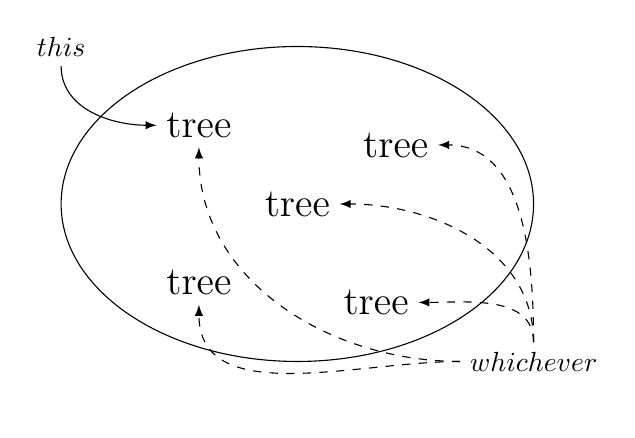
\begin{tikzpicture}
		\node (ellipse)	at (3,2)	{};
		\node (this)	at (0,4)	{$this$};
		\node (some)	at (6,0)	{$whichever$};

		\node (fig_1)	at (2-0.25 , 3+0.00)	{\Large\faicon{tree}};
		\node (fig_2)	at (4+0.25 , 3-0.25)	{\Large\faicon{tree}};
		\node (fig_3)	at (2-0.25 , 1+0.00)	{\Large\faicon{tree}};
		\node (fig_4)	at (4+0.00 , 1-0.25)	{\Large\faicon{tree}};
		\node (fig_5)	at (3-0.00 , 2+0.00)	{\Large\faicon{tree}};

		\draw (ellipse) ellipse [x radius=3, y radius=2];

		\draw[-latex] (this) to [out=south, in=west] (fig_1);
		\draw[-latex, dashed] (some) to [out=west, in=south] (fig_1);
		\draw[-latex, dashed] (some) to [out=north, in=east] (fig_2);
		\draw[-latex, dashed] (some) to [out=west, in=south] (fig_3);
		\draw[-latex, dashed] (some) to [out=north, in=east] (fig_4);
		\draw[-latex, dashed] (some) to [out=north, in=east] (fig_5);
	\end{tikzpicture}
	}
\xe

Thus, the functional definition for \rayr{me/}{mə-} should look as given in 
(\ref{ex:memorphlex}): the NP it is added to is neither definite a definite nor
specific reference, the speaker means just any representative of the kind the
nominal head specifies.

\begin{morphlex}
\ex\label{ex:memorphlex}%
\adjustbox{valign=t}{%
	\begin{tabu} {\usetabu{morphlexnarrow}}
	\rayr{\larger me/}{mə-}
		& Cl
		& \begin{tabular}[t]{l l l}
			\ups{\Def} & = & $-$ \\
			\ups{specific} & = & $-$ \\
		\end{tabular}
	\end{tabu}%
}
\xe
\end{morphlex}

Since according to \citet[152]{lyons1999}, demonstratives are inherently
definite---and their reference is specific, too---the deictic proclitics
\xayr{Ed/}{eda-}{this}, \xayr{Ad/}{ada-}{that}, and \xayr{d/}{da-}{such} are in
complementary distribution with the inspecificity marker, as demonstrated by
(\ref{ex:inspecdeix}): neither combination of \rayr{me/}{mə-} and \rayr{Ed/}
{eda-} in (\ref{ex:inspecdeix}cd) results in an ungrammatical sentence because 
\rayr{Ed/}{eda-} encodes [\Def{}~$+$, \textsc{specific}~$+$] while \rayr{me/}
{mə-} encodes [\Def{}~$-$, \textsc{specific} $-$]. Attempting to assign
opposing values to the same feature (\Def{} and \textsc{specific},
respectively) must fail, since these cannot be united at the functional level.

\pex\label{ex:inspecdeix}
\a\label{ex:inspecdeix_1}\begingl
	\gla Ang nakasyon nihanye eda-mehirya. //
	\glb ang nakas-yon nihan-ye-Ø eda=mehir-ya //
	\glc \AgtT{} grow-\TplN{} fruit-\Pl{}-\Top{} this=tree-\Loc{} //
	\glft `Fruits are growing on this tree.' //
\endgl

\a\label{ex:inspecdeix_2}\begingl
	\gla Ang nakasyon nihanye mə-mehirya. //
	\glb ang nakas-yon nihan-ye-Ø mə=mehir-ya //
	\glc \AgtT{} grow-\TplN{} fruit-\Pl{}-\Top{} whichever=tree-\Loc{} //
	\glft `Fruits are growing on whichever tree.' //
\endgl

\a\ljudge*\label{ex:inspecdeix_3}\begingl
	\gla Ang nakasyon nihanye mə-eda-mehirya. //
	\glb ang nakas-yon nihan-ye-Ø mə=eda=mehir-ya //
	\glc \AgtT{} grow-\TplN{} fruit-\Pl{}-\Top{} whichever=this=tree-\Loc{} //
\endgl

\a\ljudge*\label{ex:inspecdeix_4}\begingl
	\gla Ang nakasyon nihanye eda-mə-mehirya. //
	\glb ang nakas-yon nihan-ye-Ø eda=mə=mehir-ya //
	\glc \AgtT{} grow-\TplN{} fruit-\Pl{}-\Top{} this=whichever=tree-\Loc{} //
\endgl

\xe

The inspecificity proclitic \rayr{me/}{mə-} cannot commonly be combined with
pronouns, since personal pronouns as well as demonstrative pronouns have a
definite reference; combining the clitic with an indefinite pronoun would be
redundant. With interrogative pronouns it is feasible to use \rayr{me/}{mə-} as
an intensifier, though without the vulgar tone of the English translation given
in the following example:

\ex\label{ex:meinter}\begingl
	\gla Amangreng mə-simin? //
	\glb amang=reng mə=simin //
	\glc happen=\TsgI{}.\Aarg{} whichever=how //
	\glft `How the fuck did that happen?' //
\endgl\xe

\subsubsection{Quantifying clitics}

As described in \autoref{clitics_quant} (p.~\pageref{clitics_quant}~ff.) and 
\autoref{subsec:quantifiers}, Ayeri has a number of suffixed---that is,
enclitic---quantifiers which can attach to inflected nouns. These, along with
their non-clitic counterparts, are modifiers and are thus part of an NP's list
of adjuncts, \Adjc{}, along with adjectives and nominal adjuncts. An example of
this is given in (\ref{ex:nounquantavm}), using the clitic quantifier
\xayr{/iknF}{-ikan}{much, many; very}. Since the quantifier already lexically
expresses a multitude in this case, the noun does not carry redundant plural
marking.

\pex\label{ex:nounquantavm}
\a\label{ex:nounquantavm_1}\begingl
	\gla Sa tahayeng bisuay-ikan ban //
	\glb sa taha=yeng bisuay.Ø=ikan ban //
	\glc \PatT{} have=\TsgF{}.\Aarg{} idea.\Top{}=many good //
	\glft `She has many good ideas.' //
\endgl

\a\label{ex:nounquantavm_2}
\begin{avm}
\[
%	\Pred	&	\astruct{have}{\ups{\Subj}, \ups{\Obj}} \\
	\Top	&	\[
					\Pred	&	`idea' \\
					\Anim	&	$+$ \\
					\Case	&	\Parg \\
					\Adjc	&	\{
									\[
										\Pred	&	`many' \\
									\], \\
									\[
										\Pred	&	`good' \\
									\]
								\}
				\] \tikzmark{nounquantavm_top} \\

	% \Subj	&	\[
	% 				\Pred	&	`pro' \\
	% 				\Anim	&	$+$ \\
	% 				\Case	&	\Aarg \\
	% 				\Gend	&	\F \\
	% 				\Num	&	\Sg \\
	% 				\Pers	&	\Third \\
	% 			\] \\

	\Obj	&	\tikzmark{nounquantavm_obj} \\
\]
\end{avm}

\begin{tikzpicture}[remember picture, overlay]
\draw [rounded corners=1ex] ([yshift=1ex]{pic cs:nounquantavm_top})
	-- ++(east:1em) |- ([yshift=1ex]{pic cs:nounquantavm_obj}););
\end{tikzpicture}

\xe

Clitic quantifiers as well can combine at least with independent personal
pronouns especially in the plural, and demonstrative pronouns. A clitic
quantifier can also still be recognized in the interrogative pronoun 
\xayr{siknF}{sikan}{how many}, although here it is incorporated into the
pronoun itself, that is, there is no productive combination of interrogative
pronouns and quantifiers, with the exception of \xayr{sinY}{sinya}{who}. With
indefinite pronouns, quantifiers are somewhat redundant in some combinations,
though it is feasible in this regard to use them for emphasis. The relativizer
\rayr{si}{si} and its declined forms cannot be quantified; the simple and most
common form of the relativizer, \rayr{si}{si}, is also unstressed, which makes
it a bad host for a clitic. Combinations of pronouns and quantifying clitics
are illustrated in (\ref{ex:proquant}).

\pex\label{ex:proquant}
\a\label{ex:proquant_perspro}\begingl
	\gla Ang koronay tas-ikan. //
	\glb ang koron=ay.Ø tas=ikan //
	\glc \AgtT{} know=\Fsg{}.\Top{} \TplM{}.\Parg{}=many //
	\glft `I know many of them.' //
\endgl

\a\label{ex:proquant_dempro}\begingl
	\gla Kalam adanyana-ikoy //
	\glb kalam adanya-na=ikoy //
	\glc true that.one-\Gen{}=not.much //
	\glft `Little about that is true.' //
\endgl

\a\label{ex:proquant_interpro}\begingl
	\gla Yomāra sinyareng-ma? //
	\glb yoma-ara sinya-reng=ma //
	\glc exist-\TsgI{} what-\AargI{}=enough //
	\glft `What is there enough of?' //
\endgl

\a\label{ex:proquant_indefpro_1}\begingl
	\gla Ang ilye {} @ Pada enyaley-kay cam. //
	\glb ang il-ye Ø= Pada enya-ley=kay cam //
	\glc \Aarg{} give-\TsgF{} \Top{}= Pada everything-\PargI{}=a.little 
		\TplM{}.\Dat{} //
	\glft `Pada gave them a little of everything.' //
\endgl

\a\label{ex:proquant_indefpro_2}\begingl
	\gla Enyāng-hen siyan? //
	\glb enya-ang=hen siyan //
	\glc everyone-\Aarg{}=all where //
	\glft \textit{Literally:} `Where is all of everyone?' //
\endgl

\a\label{ex:proquant_relpro}\ljudge*\begingl
	\gla Le inttang piyu si-ma ya yomareng bukuno. //
	\glb le int=tang piyu-Ø si=ma ya yoma-reng bukuno-Ø //
	\glc \PargI{} buy=\TplM{}.\Aarg{} grain-\Top{} \Rel{}=enough \LocT{}
	exist=\TsgI{}.\Aarg{} storage-\Top{} //
	\glft \textit{Intended:} `They are buying the grain enough of which is 
		in the storage' //
\endgl

\xe

\section{Adjective and adverb phrases}
\label{sec:adjps-advps}

Adjectives and adverbs in Ayeri are largely similar in that they can both be
modified by adverbs like \fw{very}, and they both modify heads: adjectives
modify nouns, adverbs modify everything else. \citet[51]{carnie2013} urges his
readers to think about whether it is sensible to distinguish between the two
categories, so let us focus in this section on structural similarities and
dissimilarities between the two, as well as their distribution as morphemes.

\subsection{Adjective phrases}
\label{subsec:adjps}

As described in the previous section, APs are usually found as adjuncts of NPs
or DPs, where they describe properties of these nominal elements. Adjectives
are likewise commonly found as open complements (\XCompl{}) in equative
statements, which will be dealt with in \autoref{subsec:eqs}. Possessive
pronouns can be used as adjective-like modifiers as well, though they are
probably still better classified as DP heads, since they are functional
morphemes. Possessive adjectives thus also do not share all the morphological
properties of adjectives, for instance, they cannot be compared (see
\autoref{phsec:possadj}, p.~\pageref{phsec:possadj}), also they can only be
instanced once. In other words, it is not possible to modify the same noun with
multiple possessive morphemes, which means that they are not part of \Adjc{}.
The phrase-structure rule in (\ref{ex:adjpstruct}) and the c-structure tree in
(\ref{ex:adjpcstruct}) show how an AP is constructed.

\pex\label{ex:adjpstruct}
\a AP → \anno*{\xbar{A}}
\a \xbar{A} → \anno*{\xhead{A}} $\left(\anno*[{\pass{\GF}}]{XP}\right)$
\xe

\ex~\label{ex:adjpcstruct}\labels
\begin{forest}
[{\anno[\{\pass{\Adjc} | \pass{\XCompl}\}]{AP}}
	[\anno{\xbar{A}}
		[\anno{\xhead{A}}]
		[{$\left(\anno[{%
				\pass{\GF}%
			}]{XP}\right)$%
		}]
	]
]
\end{forest}
\xe

Adjective phrases have an adjective as their lexical head. This head may be
extended by modifiers adjoined to \xbar{A}; \xbar{A} repeats for the adjunction
of multiple modifiers. Since modifiers follow their heads here as well, APs are
also a right-branching constituent. Modifiers of adjectives are subsumed under
the label XP here, which here stands for AdvP, NP, DP, PP, and CP. An example
of each phrase type modifying an adjective is given in (\ref{ex:adjmod}).

\pex\label{ex:adjmod}
\a\label{ex:adjmod_adv}%
	\begin{minipage}[t]{.667\remaining}%
	\begingl
		\glpreamble adjective + AdvP: //
		\gla Adareng bisuayas sadayo kalam. //
		\glb ada-reng bisuay-as sadayo kalam //
		\glc that-\AargI{} idea-\Parg{} crazy truly //
		\glft `That is a truly crazy idea.' //
	\endgl~\\

	\begin{avm}
	\[
		\Adjc		&	\{\[
			\Pred	&	`crazy` \\
			\Adjc	&	\{\[
				\Pred	&	`truly' \\
			\]\} \\
		\]\} \\
	\]
	\end{avm}
	\end{minipage}
	~
	\begin{forest} narrower nodes, shorter edges, italic leaves,
	[{\anno[\pass{\Adjc}]{AP}}
		[\anno{\xbar{A}}
			[\anno{\xhead{A}}
				[sadayo]
			]
			[{\anno[\pass{\Adjc}]{AdvP}}
				[{kalam}, roof]
			]
		]
	]
	\end{forest}

\a\label{ex:adjmod_np}%
	\begin{minipage}[t]{.667\remaining}
	\begingl
		\glpreamble adjective + NP: //
		\gla Yang mino yanena nā. //
		\glb yang mino yan-ena nā //
		\glc \Fsg{}.\Aarg{} happy son-\Gen{} \Fsg{}.\Gen{} //
		\glft `I am happy about my son.' //
	\endgl~\\

	\begin{avm}
	\[
		\XCompl	&	\[
			\Pred		&	`happy' \\
			\Oblq{src}	&	\[
				\Pred	&	`son' \\
				\Case	&	\Gen \\
				\Poss	&	\[
					\Pred	&	`$pro$' \\
					\Case	&	\Gen \\
					\Num	&	\Sg \\
					\Pers	&	\First \\
				\] \\
			\] \\
		\] \\
	\]
	\end{avm}
	\end{minipage}
	~
	\begin{forest} narrower nodes, shorter edges, italic leaves,
	[{\anno[\pass{\XCompl}]{AP}}
		[\anno{\xbar{A}}
			[\anno{\xhead{A}}
				[mino]
			]
			[{\anno[\pass{\Oblq{src}}]{NP}}
				[{yanena nā}, roof]
			]
		]
	]
	\end{forest}\medskip

\a\label{ex:adjmod_dp}%
	\begin{minipage}[t]{.667\remaining}
	\begingl
		\glpreamble adjective + DP //
		\gla Yang mino kalam vayam. //
		\glb yang mino kalam vayam //
		\glc \Fsg{}.\Aarg{} happy really \Second{}.\Dat{} //
		\glft `I am really happy for you.' //
	\endgl~\\

	\begin{avm}
	\[
		\XCompl	&	\[
			\Pred	&	`happy' \\
			\Adjc	&	\{\[
				\Pred	&	`really' \\
			\]\} \\
			\Oblq{goal}	&	\[
				\Pred	&	`$pro$' \\
				\Case	&	\Dat \\
				\Num	&	\Sg \\
				\Pers	&	\Second \\
			\] \\
		\] \\
	\]
	\end{avm}
	\end{minipage}
	~
	\begin{forest} narrower nodes, shorter edges, italic leaves,
	[{\anno[\pass{\XCompl}]{AP}}
		[\anno{\xbar{A}}
			[\anno{\xbar{A}}
				[\anno{\xhead{A}}
					[mino]
				]
				[{\anno[\pass{\Adjc}]{AdvP}}
					[{kalam}, roof]
				]
			]
			[{\anno[\pass{\Oblq{goal}}]{DP}}
				[{vayam}, roof]
			]
		]
	]
	\end{forest}\medskip

\a\label{ex:adjmod_pp}%
	\begin{minipage}[t]{.667\remaining}
	\begingl
		\glpreamble adjective + PP //
		\gla Yāng petau kong padangya yana. //
		\glb yāng petau kong padang-ya yana //
		\glc \TsgM{} stupid inside mind-\Loc{} \TsgM{}.\Gen{} //
		\glft `He is stupid inside of his mind.' //
	\endgl~\\

	\begin{avm}
	\[
		\XCompl	&	\[
			\Pred		&	`stupid' \\
			\Oblq{loc}	&	\[
				\Case	&	\Loc \\
				\Pred	&	\astruct{inside}{\ups{\Obj}} \\
				\Obj	&	\[
					\Pred	&	`mind' \\
				\] \\
			\] \\
		\] \\
	\]
	\end{avm}
	\end{minipage}
	~
	\begin{forest} narrower nodes, shorter edges, italic leaves,
	[{\anno[\pass{\XCompl}]{AP}}
		[\anno{\xbar{A}}
			[\anno{\xhead{A}}
				[petau]
			]
			[{\anno[\pass{\Oblq{loc}}]{PP}}
				[{kong padangya}, roof]
			]
		]
	]
	\end{forest}\medskip

\a\label{ex:adjmod_cp}%
	\begin{minipage}[t]{.667\remaining}
	\begingl
		\glpreamble adjective + CP //
		\gla Adareng ban, da-tangyang. //
		\glb ada-reng ban da=tang=yang //
		\glc that-\TsgI{}.\Aarg{} good such=hear=\Fsg{}.\Aarg{} //
		\glft `It is good to hear this.'\\
			\textit{Literally:} `It is good I hear so.' //
	\endgl~\\

	\begin{avm}
	\[
		\XCompl	&	\[
			\Pred	&	`good' \\
			\Compl	&	\[
				\Pred	&	\astruct{hear}{\ups{\Subj}, \ups{\Obj}} \\
				... \\
			\] \\
		\] \\
	\]
	\end{avm}
	\end{minipage}
	~
	\begin{forest} narrower nodes, shorter edges, italic leaves,
	[{\anno[\pass{\XCompl}]{AP}}
		[\anno{\xbar{A}}
			[\anno{\xhead{A}}
				[ban]
			]
			[{\anno[\pass{\Compl}]{CP}}
				[{da-tangyang}, roof]
			]
		]
	]
	\end{forest}\medskip

\xe

Example (\ref{ex:adjmod_adv}) gives the f- and c-structures for the adjective
phrase to show that \Adjc{} may be recursive: an adjective which serves as one
of many modifiers to a noun can itself be modified by adverbs. Likewise, an
adjective--adverb combination can be complemented by an NP, as shown in
(\ref{ex:adjmod_dp}). Especially in (\ref{ex:adjmod_np}) and
(\ref{ex:adjmod_dp}) we can see Ayeri's propensity for using cases with
complements where English would use prepositions. Thus, in
(\ref{ex:adjmod_np}), `about' is expressed by putting the nominal complement in
the genitive case: the NP complement expresses the source by which the
experiencing subject becomes proud. This, however, should not be conflated with
a possessor, \Possr{}, but should be labeled separately as an oblique
complement, \Oblq{src}. Similarly, the recipient of the subject's happiness
appears as an NP complement in the (ethical) dative in (\ref{ex:adjmod_dp}).
Instrumental and causative NP complements instead of PPs may be found as well.
Since in \Lfg{}, empty \xbar{X} nodes are collapsed, \Lfg{}'s version of X-bar
theory does not strictly distinguish between complements and adjuncts
\citep[127, footnote 52]{bresnan2016}; the functional annotation provides
information about whether a sister node to \xhead{X} is a complement or an
adjunct instead.

As pointed out in \autoref{sec:adjectives}, Ayeri's adjectives inflect very
little, since there is no agreement morphology. However, it is possible for
adjectives to be compared and to be negated by means of morphology. This is
reflected in the functional annotations given in (\ref{ex:adjmorphlex}). The
features \Compar{} and \Neg{} appear in brackets here, since they do not
apply to every adjective: adjectives normally appear in the positive in both
regards, comparison and polarity, and are morphologically unmarked in these
cases.

\begin{morphlex}
\ex\label{ex:adjmorphlex}%
\adjustbox{valign=t}{%
	\begin{tabu} {\usetabu{morphlexnarrow}}
	...
		& A
		& \begin{tabular}[t]{l l l}
			\ups{\Pred} & = & `...' \\
			(\ups{\Compar} & = & \{\Comp, \Supl\}) \\
			(\ups{\Neg} & = & $+$) \\
		\end{tabular}
	\end{tabu}%
}
\xe
\end{morphlex}

Examples of the different ways an adjective may be morphologically marked and
their respective representation as an \Avm{} are given in (\ref{ex:adjmorph}).

\pex\label{ex:adjmorph}
\a\label{ex:adjmorph_compar}
\begin{minipage}[t]{.5\remaining}
\begingl
	\gla nake-vā //
	\glb nake=vā //
	\glc tall=\Supl{} //
	\glft `tallest' //
\endgl
\end{minipage}
~
\begin{avm}
\[
	\Pred	&	`tall' \\
	\Compar	&	\Supl \\
\]
\end{avm}

\a\label{ex:adjmorph_neg}
\begin{minipage}[t]{.5\remaining}
\begingl
	\gla mingoy //
	\glb ming-oy //
	\glc capable-\Neg{} //
	\glft `incapable' //
\endgl
\end{minipage}
~
\begin{avm}
\[
	\Pred	&	`capable' \\
	\Neg	&	$+$ \\
\]
\end{avm}

\a\label{ex:adjmorph_compar+neg}
\begin{minipage}[t]{.5\remaining}
\begingl
	\gla pasīsoy-eng //
	\glb pasīsa-oy=eng //
	\glc interesting-\Neg{}=\Comp{} //
	\glft `more uninteresting' //
\endgl
\end{minipage}
~
\begin{avm}
\[
	\Pred	&	`interesting' \\
	\Compar	&	\Comp \\
	\Neg	&	$+$ \\
\]
\end{avm}

\xe

As described before (\autoref{subsec:adjcomp}), the morphemes used for
synthetic comparison of adjectives are grammaticalized clitics literally
meaning `rather, more' (\rayr{/ENF}{-eng}) and `most' (\rayr{/vaa}{-vā}) as
lexical quantifiers. With adjectives, there is no clear-cut line between their
functional and their lexical use. I have analyzed them here as functional,
since they may be interpreted as such, depending on the context. As we have
observed before (\autoref{subsec:quantifiers}), quantifier clitics may modify
adjectives like any other adverbial modifiers, except that their surface form
is clitic rather than free. Quantifying adverbs, both enclitic and free, thus
also find themselves in \Adjc{}.

\pex\label{ex:adjquant3}
\a
\begin{minipage}[t]{.5\remaining}
\begingl
	\gla luyu-mas //
	\glb luyu=mas //
	\glc strange=kind.of //
	\glft `kind of strange' //
\endgl
\end{minipage}
~
\begin{avm}
\[
	\Pred	&	`strange' \\
	\Adjc	&	\{\[
					\Pred	&	`kind of' \\
				\]\} \\
\]
\end{avm}

\a\label{ex:adjadvconv}
\begin{minipage}[t]{.5\remaining}
\begingl
	\gla valuy ipan. //
	\glb valuy ipan //
	\glc glad extremely //
	\glft `extremely glad' //
\endgl
\end{minipage}
~
\begin{avm}
\[
	\Pred	&	`glad' \\
	\Adjc	&	\{\[
					\Pred	&	`extremely' \\
				\]\} \\
\]
\end{avm}

\xe

\subsection{Adverb phrases}
\label{subsec:advps}

Adverbs, as (\ref{ex:adjadvconv}) shows, can easily be converted from
adjectives. Thus, \xayr{IpnF}{ipan}{extreme}, which is normally an adjective,
is used there in an adverbial way, meaning `extremely'. The word stays the
same, however: \rayr{IpnF}{ipan}, without a derivative affix akin to English
\fw{-ly} or French \fw{-ment}. Since adverbs and adjectives are largely similar
in that they provide additional information about the nature or circumstance of
a noun or another part of speech, \citet{carnie2013} poses the question whether
adjectives and adverbs should be better analyzed as being part of the same
category. He reasons that

\blockcquote[51]{carnie2013}{Both Adj and Adv can be modified by the word
\fw{very}, and they both have the same basic function in the grammar---to
attribute properties to the items they modify. In fact, the only major
distinction between them is syntactic: Adjectives appear inside NPs, while
adverbs appear elsewhere.}

Adjectives and adverbs are in complementary distribution, which, he writes,
would normally be taken as evidence that these two things are of the same
category. In fact, the only reason \citet{carnie2013} adduces for keeping the
two categories apart is \textquote{because they are familiar to most people},
and he prompts the reader to consider that uniting them in a single
supercategory \textcquote[51]{carnie2013}{might provide a better analysis and
might be better motivated scientifically}. \citet[126]{bresnan2016} also
classify both adjectives and adverbs as heads of AP with reference to
\citet{emonds1976}. As described in \autoref{sec:adverbs}, the only morphology
attributive adverbs take in Ayeri is comparison morphology and negation. This
is the same as with adjectives indeed, hence the functional specifications
appear equal:

\begin{morphlex}
\ex\label{ex:advmorphlex}%
\adjustbox{valign=t}{%
	\begin{tabu} {\usetabu{morphlexnarrow}}
	...
		& A
		& \begin{tabular}[t]{l l l}
			\ups{\Pred} & = & `...' \\
			(\ups{\Compar} & = & \{\Comp, \Supl\}) \\
			(\ups{\Neg} & = & $+$) \\
		\end{tabular}
	\end{tabu}%
}
\xe
\end{morphlex}

If we look at the phrase structure (\ref{ex:advpstruct}) and the c-structure
(\ref{ex:advpcstruct}) for adverbs, however, there is a slight difference in
that adverbs cannot serve as \XCompl{} in equative statements; they also can
only be modified by other adverbs, but not by NP, DP, or CP.\footnote{For
adjectives, compare (\ref{ex:adjpstruct}), (\ref{ex:adjpcstruct}), and
(\ref{ex:adjmorphlex}) in \autoref{subsec:adjps}.} On the other hand,
adjectives are restricted to nominal contexts whereas adverbs may modify any
other lexical category: verbs, adjectives, prepositions, as well as other
adverbs.

\pex\label{ex:advpstruct}
\a AdvP → \anno*{\xbar{Adv}}
\a \xbar{Adv} → \anno*{\xhead{Adv}} $\left(\anno*[{\pass{\Adjc}}]{AdvP}\right)$
\xe

\ex~\label{ex:advpcstruct}\labels
\begin{forest}
[{\anno[\pass{\Adjc}]{AdvP}}
	[\anno{\xbar{Adv}}
		[\anno{\xhead{Adv}}]
		[{$\left(\anno[{%
				\pass{\Adjc}%
			}]{AdvP}\right)$%
		}]
	]
]
\end{forest}
\xe

...

% \section{Adpositional phrases}
% \label{sec:pps}

% ...

% \section{Inflectional and verb phrases}
% \label{sec:ips-vps}

% ...

% \subsection{Inflectional phrases}
% \label{subsec:ips}

% ...

% \subsection{Verb phrases}
% \label{subsec:vps}

% ...

% \subsection{Equative statements}
% \label{subsec:eqs}

% ...

% * Ayeri's unmarked word order is essentially VSO, maaaaaaaybe like this???
%
%   IP
%     \
%      I'
%     /  \
%    D°   I'
%        /  \
%       I°   S
%           / \
%          NP XP*
% 
%   → Analysis similar to the one suggested for Irish by ??? and ??? 
%     (Kroeger 1991, 1993; Bresnan 2016)
%   → Probably one has to distinguish clauses with IP from `small clauses' 
% 	  (cf. exposition to Kroeger 1991) with only S
%   → S is likely an exocentric category
% 	  → support/tests for this?
% 	  → Kroeger 1991 should list some criteria in this respect
% * Subject vs. Topic vs. Actor vs. Nominative in Ayeri, in relation to
%   superficial (?) similarities with Austronesian alignment (Kroeger 1991,
%   1993, 2007; Schachter 2015)
%   → Promoting patient in whatever way does not demote logical subject etc.
%   → Ayeri's notion of A = logical subject (also what LFG calls `SUBJ', right?)
%     probably stronger than Tagalog's
%   → PROBLEM: terminology all about the place---may have inspired differences 
%     between Ayeri and real-world AA + my only now beginning to learn more
%     about syntax and stuff
%     → IMPORTANT: how do I use the respective terms and why?
% * Bresnan (2016) on extended head principle relevant w/r/t placement of 
%   finite verb in I°?
%   → Are there any tests for whether there's a covert VP after all? Nothing
%     verbal ever seems to occur in S'
%   → Ayeri should treat logical subjects and objects similarly, so no 
%     hierarchy between them?
% * Interesting problem: subject pronoun citics as a specifier of S?
%   → Funny stuff happens when adverbs are present
%   → Especially with patient-pronoun subjects (if that term is appropriate)
% * Patient subjects, causative constructions, no secundative, avoidance (?) of 
%   raising all need to be investigated with regards to proto-role mapping in 
%   a-structure ([±r, ±o])
% * Existential vs. predicative statements
%   → also, object predicatives!
%   → also, comparative verbs: kama-, eng-, va- and why they're weird
% * Agreement with conjoined/disjoined NPs
%   → due to the way verb agreement in general works, closest-conjunct agreement
%     is the most likely strategy for gender mismatches; yet number resolution.
%   → default gender for anaphoric reference to mixed-gender NPs (also animacy
%     mismatches!)
%
% \citet[153--156, 165]{bresnan2016} → pronouns to clitics to agreement
% \citet[157]{bresnan2016} → evidence criteria for IP
% \citet[151\psqq]{dixon2012} → subjects
% \citet[116\psqq]{comrie1989} → subjects
% \citet[26--54]{kroeger1991} → subjects (and actually the whole thesis)

% \section{Complementizer phrases}
% \label{sec:cps}

% ...

% \subsection{Relative clauses}
% \label{subsec:relcs}

% ...

% \subsection{Conditional clauses}
% \label{subsec:condcs}

% ...

% \subsection{Other types}
% \label{subsec:cps_other}

% ...
